%!TEX root = /home/renaud/Documents/EPL/tfe/latex/tfe.tex
\chapter{Numerical Considerations} \label{chap:numerical}
\textcolor{red}{À retravailler une fois le travail fini.}
The final goal of this work is to develop a simpler box-model of the overturner model, where the boxes are determined via a community detection method. In order to apply such a community detection method, the solution to the overturner transport model \eqref{eq:C_PDE_vec} must be computed at different times and for different initial conditions. However, equation \eqref{eq:C_PDE_vec} cannot be solved analytically so that numerical methods must be resorted to. A lot of different numerical methods have been developed through the years, each having their pros and cons. Here, we briefly summarize the main types of methods available, with their main advantages and disadvantages. This allows then to make an informed decision about which method to use in this work. Most of the discussion in the following paragraphs is inspired from \cite{spivakovskaya2007lagrangian} and \cite{spivakovskaya2007backward}. 

A very popular class of numerical methods is formed by the Eulerian methods, in which the advection-diffusion equation is solved on a fixed spatial grid. This class encompass the finite difference method, finite element method and finite volume method. A second class is formed by the Lagrangian methods, where particles are followed through space at every time step. As we shall see later, the movement of an individual particle is modeled with a stochastic differential equation (SDE) which is consistent with the advection-diffusion equation. The idea is to estimate the concentration by simulating the trajectories of a large number of particles and taking averages. Several averaging methods have been developed to estimate the concentration from the set of particles positions: we shall come back to this further in section \ref{boxcounting_kernel}. Finally, a third class of mixed Eulerian-Lagrangian methods has been developed, which basically attempts to combine the advantages of both approaches. Such conceptually attractive methods have been widely applied in applications. They are however more complex to implement; in view of the relative simplicity of the overturner problem, we will not consider such mixed methods here.

Both Eulerian and Lagrangian methods have their own advantages and disadvantages. The Eulerian methods provide the convenience of a fixed grid and are easy to implement. The main drawbacks are the inherent dispersion errors and artificial oscillations, leading to solutions that may be neither mass conservative nor positive \cite{stijn1987positive}, \cite{yang1998accuracy}. Basically, the effect of dispersion errors is similar to physical dispersion but it is due to truncation errors. Artificial oscillations are typical from higher order methods designed to reduce dispersion errors. Those downsides could become excessively severe in case of problems involving a sharp concentration front, for instance advection-dominated problems or problems with large gradients on the initial concentration field (typically delta-like initial concentration) \cite{zheng2002applied}. In those cases, numerical dispersion (i.e. dispersion due to dispersion errors) tends to inappropriately smooth out the sharp concentration front, whereas artificial oscillations tends to become more important, leading to serious problem with the positiveness of the solution. 

On the other hand, Lagrangian methods ensures that the solution is always mass conservative and nonnegative. They are thus more suited than Eulerian methods to advection-dominated problems and to problems with large concentration gradients, since they do not suffer from dispersion errors and artificial oscillations. Moreover, if the tracer does not occupy the whole domain, the Lagrangian methods may be computationally more efficient than their Eulerian counterpart \cite{hunter1987application}. Depending on the number of particles used, Lagrangian methods may also require less storage than finite differences or finite element methods. Another advantage of Lagrangian methods is that they make it possible to advect the particles exactly when  the velocity field can locally be described by an analytical function \cite{hunter1993use}. Finally, because each realization of the particle movement is independent from the others, Lagrangian methods are perfect candidates for parallelization. For instance, the MPI library makes it pretty easy and efficient to parallelize a code based on random walk models. Among the drawbacks of particle methods, the lack of a fixed grid may lead to numerical instability and computational difficulties \cite{yeh1990lagrangian}. If flow variables are not known analytically, their interpolation to the particle location could lead to local mass balance errors and solution anomalies \cite{labolle1996random}. Finally, the number of particles needed to get a smooth solution might be large leading to a large computational time, but this can be compensated by a parallelization of the code.

Considering the above discussion, it seems that a Lagrangian method is more appropriate for our concern. Indeed, in order to build an approximation of the transition probability matrix, the domain $\Omega$ is partitioned into grid cells or boxes. For a simulation time $T$, an entry $[\b M(T)]_{ij}$ is the probability that a particle goes from box $i$ to box $j$ in a time $T$. To estimate the entries of a line $i$ of the matrix, the idea is to run a simulation for a time $T$ and an initial concentration which is uniform in box $i$ and zero in every other box. The initial concentration is thus sharp, a first argument in favor of a Lagrangian method. Furthermore, the concentration is interpreted as a probability, hence positiveness and mass conservation are crucial topics, another point for Lagrangian methods. Finally, the flow variables are in our case known analytically, which considerably reduce the drawbacks of Lagrangian methods pointed out above. For these reasons, we choose to go for a Lagrangian method. 
% Concentration initiale sharp
% concentration interprétée comme une proba -> positiveness & mass conservation ++
% flow variables known analytically : dans ce cas la plupart des désavantages exprimés ci-dessus sont sans objet
%!TEX root = /home/renaud/Documents/EPL/tfe/latex/tfe.tex
\section{Preliminaries}
We introduce here the notions of stochastic differential equations (SDE's) and stochastic integrals. Those are the fundamental tools at the basis of the Lagrangian numerical methods. The discussion that comes next is based on several references, including \cite{gardiner1985stochastic}, \cite{heemink2011slides}, \cite{keunings} and \cite{spivakovskaya2007lagrangian}. Other references have been used for local parts of the work; they are then cited when they come in handy. Some results are stated without proofs. In such cases, unless otherwise stated, the reader may refer to \cite{gardiner1985stochastic} for formal proofs.

The idea behind Lagrangian methods is to estimate the concentration obeying an advection-diffusion-reaction equation by simulating the trajectories of a large number of particles in the flow. In this work, we restrict ourselves to advection diffusion equations of the form \eqref{eq:C_PDE_vec}, which we recall here for the sake of readability:
\begin{equation} \label{eq:ADE}
	\frac{\partial C}{\partial t} = \nabla \cdot (-\b u C + \b K \nabla C)
\end{equation}
In the next, equation \eqref{eq:ADE} will be referred to as the \textit{transport model}. In order to implement a numerical method tracking the fates of individual particles, an equation describing the fate of such a particle must be derived, and that equation must be consistent with the transport model. Formally, the transport model can be interpreted as a Fokker-Planck equation, namely the partial differential equation governing the time evolution of the probability density function $p(\b x,t)$ of the position of a particle. The correspondence is made by interpreting the concentration as the probability density function: $p=C$. 

At the microscopic scale, Brownian diffusion is modeled by a stochastic force acting on the particles. This force is interpreted as the resultant of atomic bombardment on the particle. Intuitively, the direction of the force due to atomic bombardment is constantly changing, and at different times the particle is hit more on one side than another, leading to the seemingly random nature of the force, and hence of the motion. Therefore, the differential equation governing the position $\b x(t)$ of a particle is stochastic. For example, Langevin proposed in 1908 an equation governing the position of a Brownian particle, which in 1D can be written in the form :
\begin{equation} \label{eq:Langevin}
	\frac{dx}{dt} = a(x,t) + b(x,t)\xi(t),
\end{equation}
where $x$ is the position of the particle, $a(x,t)$ and $b(x,t)$ are known functions and $\xi(t)$ is the rapidly fluctuating random term. The simplest model is obtained by considering that $\xi(t)$ is a white noise, i.e.
\begin{subnumcases}{}
		\esp{\xi(t)} = 0,\\
		\esp{\xi(t)\xi(t')} = \delta(t-t'),
\end{subnumcases}
where $\esp{\cdot}$ denotes expectation. The fact that $\xi$ has zero mean is because any nonzero mean can be absorbed in the term $a(x,t)$. The second condition states that $\xi(t)$ is uncorrelated, namely that the random force acting on a particle at a time is independent of the random forces acting on that particle at any other time. This simple form of the noise is of course an unrealistic idealization of the atomic bombardment force. It is possible to show that
\begin{equation} \label{eq:whitenoise_integral}
	\int_0^t \xi(t') \rm dt' = W(t),
\end{equation}
where $W(t)$ is the \textit{Wiener process}, a \textit{continuous} stochastic process defined by the following characteristics:
\begin{subnumcases}{\label{eq:WienerProcess}}
	W(0) = 0,\\
	W(t_2) - W(t_1)  \sim \mathcal{N}(0,t_2-t_1),\\
	\esp{[W(t_4)-W(t_3)][W(t_2)-W(t_1)]} = 0, \label{eq:independent_inc}
\end{subnumcases}
where $t_1 < t_2 < t_3 < t_4$. In other words, $W(t)$ is a zero mean gaussian process of variance $t$ which has the property of independent increments. Suppose now that $a(x,t) = a$ and $b(x,t) = b$ are constant. The above relations imply that the solution to $\eqref{eq:Langevin}$ is
\begin{equation}
	x(t) = at + bW(t),
\end{equation}
where we implicitly assumed that $x(0) = 0$. However, one can show that the Wiener process is not differentiable with probability 1. We are thus faced with a paradox here since this implies that $x(t)$ is itself non-differentiable, and hence that the Langevin equation as stated in \eqref{eq:Langevin} \textit{does not exist mathematically}. In fact, $\xi(t)$ is the derivative of $W(t)$ in the \textit{distributive sense}. From \eqref{eq:whitenoise_integral}, it follows directly that
\begin{equation}\label{eq:dW}
	\rm dW(t) \equiv W(t+\rm dt) - W(t) = \xi(t) \rm dt,
\end{equation}
but it is incorrect (or at least very misleading) to write $\frac{dW(t)}{dt} = \xi(t)$, since the Wiener process is nowhere differentiable with probability 1, as already stated above.

Hopefully this introductory example shows the need for some preliminary steps in order to rigorously define a Stochastic Differential Equation (SDE), and to formalize the link between SDE's and Fokker-Planck equations. This is precisely the goal of the next pages.

\subsection{Formal definition of a SDE}
In this section, we restrict ourselves to a one-dimensional problem. This allows to make the notations less cumbersome while still introducing all the tools and concepts that are needed in order to understand the two-dimensional Lagrangian model which is at the basis of our numerical resolution of the overturner model for the meridian concentration in the Atlantic ocean. Indeed, all the results presented here can almost straightforwardly be extended to several dimensions. Consider again the Langevin equation \eqref{eq:Langevin}. We have shown in the introduction that the equation does not really make sense under that form. What we are now going to show is that the corresponding \textit{integral equation} 
\begin{equation} \label{eq:SDEint_xsi}
	x(t) = x(t_0) + \int_{t_0}^t a(x(s),s) \rm ds + \int_{t_0}^t b(x(s),s) \xi(s) \rm ds
\end{equation}
can be interpreted consistently. The first integral is a standard Lebesgue integral of a function $a$ of the stochastic process $x(t)$. The second integral has to be defined carefully, because of the presence of the white noise. By \eqref{eq:dW}, we rewrite it as
\begin{equation} \label{eq:stoch_int}
	\int_0^t b(x(s),s) \rm dW(s),
\end{equation}
which is a kind of stochastic Stieltjes integral (see appendix \ref{app:stieltjes}). Consider the partition of interval $[t_0,\,t]$:
\begin{equation}
	t_0 \le t_1 \le t_2 \le \dots \le t_{n-1} \le t_n = t,
\end{equation}
and define intermediate points $\tau_i \in [t_{i-1},\, t_i]$. Such a partition will often be used thereafter without introducing it explicitly every time it appears. The stochastic integral of $b$ with respect to the Wiener process $\int_{t_0}^t b(x(s),s) \rm dW(s)$ is defined as a mean-square limit (see appendix \ref{app:mslim}) of the partial sum
\begin{equation}
	S_n = \sum_{i=1}^n b(x(\tau_i),\tau_i) [W(t_i)-W(t_{i-1})].
\end{equation}
Such a limit is not unique: it depends on the particular choice of $\tau_i$. This sensibility to the choice of location $x(\tau_i)$ at which the function is evaluated is a consequence of the unbounded variation of the Wiener process. Popular choices are $\tau_i = t_i$, $\tau_i = \frac{1}{2}(t_{i-1}+t_i)$ or $\tau_i = t_i$, corresponding to the \textit{Itô}, \textit{Stratonovich} and \textit{backward Itô} stochastic integrals, respectively. Hence, for a stochastic integral such as \eqref{eq:stoch_int} to be well-defined, its \textit{interpretation} must be stated explicitly. Namely, one must specify if the integral is taken in the \textit{Itô}, \textit{Stratonovich} or \textit{backward Itô} sense, or any other interpretation corresponding to a given choice of $\tau_i$. Only the Itô and backward Itô interpretations will be considered in this work. To avoid any confusion, we will denote the Itô integral by $\I\int$ and the backward Itô integral by $\bI\int$. Hence
\begin{subequations}
\begin{align}
        \I\int_{t_0}^t b(x(s),s) \rm dW(s) &= \mslim_{n\rightarrow \infty} \sum_{i=1}^n b(x(t_{i-1}),t_{i-1}) [W(t_i)-W(t_{i-1})], \label{def:I}\\
        \bI\int_{t_0}^t b(x(s),s) \rm dW(s) &= \mslim_{n\rightarrow \infty} \sum_{i=1}^n b(x(t_{i}),t_{i}) [W(t_i)-W(t_{i-1})]. \label{def:bI}
\end{align}
\end{subequations}
\paragraph{Remark}\label{remark:backwardIto} In the backward Itô definition of the stochastic integral, only $x$ needs to be evaluated at $t_i$: if $b(x,t)$ is differentiable in $t$ (which is assumed here), the integral is independent of the particular choice of value for $t$ in the range $[t_{i-1},\, t_i]$. Hence, we could replace $b(x(t_i),t_i)$ by $b(x(t_i),\tau_i)$ with $\tau_i \in [t_{i-1},\, t_i]$ in the definition \eqref{def:bI}. Note that this remark is not restricted to backward Itô integration: if $b$ is differentiable in $t$, only the location $x(\tau_i)$ at which $b$ is evaluated in the sum affects the limit.

Conventionally, a stochastic differential equation such as $\eqref{eq:Langevin}$ is written in the form
\begin{equation} \label{eq:generalSDE}
	\begin{cases}
		\rm dx(t) = a(x(t),t) \rm dt + b(x(t),t) \rm dW(t),\\
		x(t_0) = x_0. 
	\end{cases}
\end{equation}
Equation \eqref{eq:generalSDE} has to be interpreted as the implicit integral equation
\begin{equation}
	x(t) = x_0 + \int_{t_0}^t a(x(s),s) \rm ds + \int_{t_0}^t b(x(s),s) \rm dW(s),
\end{equation}
and the interpretation of the stochastic integral must thus be stated. For example, one will talk about an Itô SDE or a backward Itô SDE, and the stochastic process $x(t)$ which is the solution to the SDE \eqref{eq:generalSDE} is different whether the stochastic integral is computed in the Itô or backward Itô sense.

It can be shown that an Itô stochastic integral $\I\int_{t_0}^t G(s) \rm dW(s)$ exists whenever the function $G$ is \textit{continuous} and \textit{nonanticipating} on the closed interval $[t_0,\,t]$. $G$ is a \textit{nonanticipating} function of $t$ is for all $t$ and $s$ such that $t<s$, $G(t)$ is statistically independent of $W(s)-W(t)$. This condition seems obviously satisfied for any deterministic function $b(x(t),t)$ of the stochastic process $x(t)$ obeying the SDE \eqref{eq:generalSDE}, since $x(t)$ only depends on anterior values of the Wiener process. For example, in the context of the position of a brownian particle, it is intuitively obvious that the unknown future collisions cannot affect the present position of the particle. From now on, we assume thus that we are dealing with \textit{nonanticipating} functions.

\subsection{Properties of the Itô integral}
When working with nonanticipating functions, it is possible to take advantage of the fact that $G(t_{i-1})$ is independent of $W(t_i) - W(t_{i-1})$ to derive particularly useful properties of the Itô integral. Such properties are generally not true for Stratonovich or backward Itô integrals. However, there is a formula called Ito's formula that allows to build rules to transform any SDE into an Itô SDE. Hence, when working with a Stratonovich or backward Itô SDE, it is often useful to transform that SDE into an equivalent Itô SDE so that the previously mentioned properties can be applied. In this section, we first derive those properties, and then we show Itô's formula for the change of variables. Those results are fundamental for connecting a SDE to the Fokker-Plank equation and for building consistent numerical schemes, as we shall see later.
\subsubsection{Rules for the differentials}
One preliminary result of first-order importance in the context of stochastic integration is that, for any nonanticipating function $G$
\begin{equation} \label{eq:dW=dt_int}
	\I\int_{t_0}^t G(s) \rm [dW(s)]^2 = \int_{t_0}^t G(s) \rm ds,	
\end{equation}
i.e. that
\begin{equation} \label{eq:dw1}
	\lim_{n\rightarrow\infty} \esp{\left(\sum_{i=1}^n G(t_{i-1})[W(t_i)-W(t_{i-1})]^2-\int_{t_0}^t G(s) \rm ds\right)^2} = 0.
\end{equation}
Let $\Delta W_i := W(t_i) - W(t_{i-1})$ and $\Delta t_i = t_i - t_{i-1}$. By the properties of the Wiener process, $\Delta W_i \sim \mathcal{N}(0,\Delta t_i)$. Hence, $\Delta W_i^2/\Delta t_i$ follows a $\chi$-squared distribution with one degree of freedom. It has thus mean $1$ and variance $2$ and thus
\begin{subequations} \label{eq:dwprop}
\begin{align}
        &\esp{\Delta W_i^2} = \Delta t_i, \quad \mbox{and} \label{eq:dwesp}\\
        &\esp{(\Delta W_i^2 - \Delta t_i)^2} = 2 \Delta t_i^2. \label{eq:dwvar}
\end{align}
\end{subequations}
Using Riemann sums, the left hand side of equation \eqref{eq:dw1} can be rewritten as
\begin{equation}
	\lim_{n\rightarrow\infty} \esp{\left(\sum_{i=1}^n G(t_{i-1})(\Delta W_i^2-\Delta t_i)\right)^2},
\end{equation}
which, by developing the square and using the linearity of the expectation operator is equal to
\begin{equation} \label{eq:dw2}
	\lim_{n\rightarrow\infty} \sum_{i=1}^n \bigg[\esp{G^2(t_{i-1})(\Delta W_i^2-\Delta t_i)^2} + \sum_{j=1}^{i-1} \esp{2G(t_{i-1})G(t_{j-1})(\Delta W_j^2 - \Delta t_j)(\Delta W_i^2 - \Delta t_i)}\bigg].
\end{equation}
Since $G$ is nonanticipating, we can use independence between terms to rewrite \eqref{eq:dw2} as
\begin{equation} \label{eq:dw3}
	\lim_{n\rightarrow\infty} \sum_{i=1}^n \bigg[\esp{G^2(t_{i-1})}\underbrace{\esp{(\Delta W_i^2-\Delta t_i)^2}}_{=2\Delta t_i^2} + \sum_{j=1}^{i-1} \esp{2G(t_{i-1})G(t_{j-1})(\Delta W_j^2 - \Delta t_j)}\underbrace{\esp{(\Delta W_i^2 - \Delta t_i)}}_{=0}\bigg],
\end{equation}
which simplifies to
\begin{equation}
	2 \lim_{n\rightarrow\infty} \sum_{i=1}^n \esp{G^2(t_{i-1})}\Delta t_i^2.
\end{equation}
If $G$ is bounded on $[t_0,\,t]$, the latter goes to zero, which concludes the proof. Since $[\rm dW(t)]^2$ only appears in the context of stochastic integration, property \eqref{eq:dW=dt_int} is often written
\begin{equation} \label{eq:dw2=dt}
	\left[\rm dW(t)\right]^2 = \rm dt,  	
\end{equation}  
but one must not forget the underlying meaning. It is important to remember that this property only holds in the context of Itô integration.

By a similar method, one can show that for any $N \ge 3$
\begin{equation}
	\left[\rm dW(t)\right]^{N} = 0,
\end{equation}
and that for any $N_1 \ge 1$, $N_2 \ge 1$
\begin{equation} \label{eq:dwdt=0}
	\left[\rm dt\right]^{N_1}\left[\rm dW(t)\right]^{N_2} = 0. 
\end{equation}

Those results are often summarized by saying that $\rm dW(t)$ is an infinitesimal of order $\frac{1}{2}$ in $\rm dt$ and that infinitesimals of order higher than $1$ are discarded when it comes to compute differentials. Intuitively, $\rm dW(t)$ is a gaussian of variance $\rm dt$; a characteristic magnitude for $\rm dW(t)$ is its standard deviation, $\sqrt{\rm dt}$ which is indeed of order $\frac{1}{2}$.

\subsubsection{The Itô formula}
Consider an arbitrary function $\phi(x(t),t)$ with $x(t)$ obeying the Itô SDE \eqref{eq:generalSDE}. We are interested in the SDE governing $\phi$. By definition, 
\begin{equation}
	\rm d\phi(x(t),t) = \phi(x(t)+\rm dx(t),t+ \rm dt) - \phi(x(t),t). 	
\end{equation}
Expanding $\phi(x(t)+\rm dx(t),t+ \rm dt)$ in Taylor series and keeping the terms up to order 1 in $\rm dt$ yields
\begin{align}
\rm d\phi(x(t),t) &= \frac{\partial \phi}{\partial t}\rm dt + \frac{\partial \phi}{\partial x}\rm dx(t) + \frac{1}{2} \frac{\partial^2 \phi}{\partial x^2} [\rm dx(t)]^2 + \dots \nonumber\\
&= \frac{\partial \phi}{\partial t}\rm dt + \frac{\partial \phi}{\partial x}\left(a(x(t),t) \rm dt + b(x(t),t) \rm dW(t)\right) + \frac{1}{2} \frac{\partial^2 \phi}{\partial x^2} \left(b^2(x(t),t) [\rm dW(t)]^2 + \dots \right) + \dots, \nonumber
\end{align}
where the derivatives are evaluated at $(x(t),t)$. Now, using that $[\rm dW(t)]^2 = \rm dt$ we get the Itô formula:
\begin{equation} \label{eq:ItoFormula}
	\rm d\phi(x(t),t) = \left[\frac{\partial \phi}{\partial t} + \frac{\partial \phi}{\partial x} a(x(t),t) + \frac{1}{2}\frac{\partial^2 \phi}{\partial x^2} b^2(x(t),t)\right] \rm dt + \frac{\partial \phi}{\partial x}b(x(t),t) \rm dW(t).
\end{equation}

\subsection{Link between Itô and backward Itô SDE's}
A same stochastic process $x(t)$ can be described both by a Itô and by a backward Itô SDE. Suppose that $x(t)$ obeys the Itô SDE
\begin{equation} \label{eq:I}
	dx(t) = a_I(x(t),t) \rm dt + b_I(x(t),t) \rm dW(t),
\end{equation}
and the equivalent backward Itô SDE
\begin{equation} \label{eq:bI}
	dx(t) = a_{bI}(x(t),t) \rm dt + b_{bI}(x(t),t) \rm dW(t). 
\end{equation}
The goal is to compute the relations between the functions $a_I$, $b_I$ and $a_{bI}$, $b_{bI}$. By \eqref{eq:bI},
\begin{equation}
	x(t) = x(t_0) + \int_{t_0}^t a_{bI}(x(s),s) \rm ds + \bI \int_{t_0}^t b_{bI}(x(t),t) \rm dW(t).
\end{equation}
Let us rewrite the backward Itô stochastic integral term
\begin{equation} \label{eq:bI-int}
	\bI \int_{t_0}^t b_{bI}(x(t),t) \rm dW(t) \triangleq \mslim_{n\rightarrow \infty} \sum_{i=1}^n b_{bI}(x(t_{i}),t_{i}) [W(t_i)-W(t_{i-1})]
\end{equation}
as an Itô integral. Since $x(t)$ satisfies the Itô SDE \eqref{eq:I}, we can apply Itô formula. This yields 
\begin{align} \label{eq:equiv1}
	b_{bI}(x(t_i),t_{i}) =~& b_{bI}(x(t_{i-1}),t_{i-1}) \nonumber\\
		&+ \left[\frac{\partial b_{bI}}{\partial t} + \frac{\partial b_{bI}}{\partial x} a_I(x(t_{i-1}),t_{i-1}) + \frac{1}{2}\frac{\partial^2 b_{bI}}{\partial x^2} b_I^2(x(t_{i-1}),t_{i-1})\right] (t_i - t_{i-1}) \nonumber\\
		&+ \frac{\partial b_{bI}}{\partial x}b_I(x(t_{i-1}),t_{i-1}) (W(t_i) - W(t_{i-1})),
\end{align}
where the derivatives are evaluated at $(x(t_{i-1}),t_{i-1})$. Introducing \eqref{eq:equiv1} in \eqref{eq:bI-int} and setting $[\rm dW(t)]^2 = \rm dt$ yields, after dropping the terms in $\rm dt \rm dW(t)$ and $\rm dt^2$:
\begin{align}
	\bI \int_{t_0}^t b_{bI}(x(t),t) \rm dW(t) =~& \mslim_{n\rightarrow \infty} \sum_{i=1}^n b_{bI}(x(t_{i-1}),t_{i-1}) [W(t_i)-W(t_{i-1})] \nonumber\\
	&+ b_I(x(t_{i-1}),t_{i-1}) \frac{\partial b_{bI}}{\partial x}[t_i - t_{i-1}],
\end{align}
and finally
\begin{equation}
	\bI \int_{t_0}^t b_{bI}(x(t),t) \rm dW(t) = \I\int_{t_0}^t b_{bI}(x(t),t) \rm dW(t) + \int_{t_0}^t b_I(x(s),s) \frac{\partial b_{bI}}{\partial x}(x(s),s) \rm ds.
\end{equation}
Therefore, we have the equivalences
\begin{equation}
	\begin{array}{ccc}
	\mbox{\underline{Itô SDE}} & & \mbox{\underline{backward Itô SDE}}\\[.2cm]
	\rm dx(t) = a_I \rm dt + b_I \rm dW(t) & \Leftrightarrow & \rm dx(t) = \left[a_I-b_I\dfrac{\partial b_I}{\partial x}\right]\rm dt + b_I \rm dW(t)
	\end{array} 	
\end{equation}
and conversely
\begin{equation} \label{eq:bI-I}
	\begin{array}{ccc}
	\mbox{\underline{backward Itô SDE}} & & \mbox{\underline{Itô SDE}}\\[.2cm]
	\rm dx(t) = a_{bI} \rm dt + b_{bI} \rm dW(t) & \Leftrightarrow & \rm dx(t) = \left[a_{bI}+b_{bI}\dfrac{\partial b_{bI}}{\partial x}\right]\rm dt + b_{bI} \rm dW(t).
	\end{array} 	
\end{equation}
Here, the dependence of $a_I$, $b_I$, $a_{bI}$ and $b_{bI}$ on $x(t)$ and $t$ have been made implicit to simplify the notations.

\subsection{Connection between Itô and backward Itô SDE's and the Fokker Planck equation}
Consider a particle in one dimension whose position $x(t)$ obeys the Itô SDE
\begin{equation} \label{eq:itoSDE}
	\begin{cases}
		\rm dx(t) = a(x(t),t) \rm dt + b(x(t),t) \rm dW(t),\\
		x(t_0) = x_0. 
	\end{cases}
\end{equation}
Let $p(x,t;y,s)$ be the probability density function of the position $x$ of the particle at time $t$ given that the particle was in position $y$ at time $s$, with $s < t$. For an infinitesimal $\rm dx$ and $\bar{x} \in \Omega$, the probability that the random variable $x(t)$ describing the position of the particle at time $t$ has value between $\bar{x}$ and $\bar{x}+\rm dx$ is given by:
\begin{equation}
	\Pr\big(\bar{x} < x(t) < \bar{x} + \rm dx \,\big|\, x(s) = y\big) = p(\bar{x},t;y,s)\rm dx.
\end{equation}
 From \eqref{eq:itoSDE} we are going the derive the partial differential equation governing the evolution of $p(x,t;x_0,t_0)$. Let $K(x)$ be an arbitrary function of $\mathcal{C}^2$ with compact support. In the next, all the derivative terms of functions $a$ and $b$ are evaluated at $(x(t),t)$ and the derivatives of $K$ are evaluated at $x(t)$, unless otherwise stated. By Itô's formula:
\begin{equation}
	\rm dK(x(t)) = \left[\frac{\partial K}{\partial x} a(x(t),t) + \frac{1}{2}b^2(x(t),t) \frac{\partial^2 K}{\partial x^2} \right] \rm dt + \frac{\partial K}{\partial x}b(x(t),t) \rm dW(t),
\end{equation}
where the derivatives are evaluated at $(x(t),t)$. Taking the expectation yields
\begin{equation}
	\esp{\rm dK(x(t))} = \esp{\frac{\partial K}{\partial x} a(x(t),t) + \frac{1}{2}b^2(x(t),t) \frac{\partial^2 K}{\partial x^2}} \rm dt,
\end{equation}
and thus
\begin{equation} \label{eq:dEKdt}
	\frac{d\esp{K(x(t))}}{dt} = \esp{\frac{\partial K}{\partial x} a(x(t),t) + \frac{1}{2}b^2(x(t),t) \frac{\partial^2 K}{\partial x^2}}.
\end{equation}
Using the probability density $p(x,t)$, we can rewrite \eqref{eq:dEKdt} as
\begin{equation} \label{eq:dEKdt_int}
	\frac{d}{dt} \int_{-\infty}^{\infty} K(x) p(x,t;x_0,t_0) \rm dx = \underbrace{\int_{-\infty}^{\infty} \frac{\partial K}{\partial x} a(x,t) p(x,t;x_0,t_0) \rm dx}_{:= I_1} + \frac{1}{2} \underbrace{\int_{-\infty}^{\infty} \frac{\partial^2 K}{\partial x^2} b^2(x,t) p(x,t;x_0,t_0) \rm dx}_{:= I_2}.
\end{equation}
Integrating $I_1$ by parts yields:
\begin{align}
	I_1 &= \left[ a(x,t)p(x,t;x_0,t_0)K(x)\right]_{-\infty}^{\infty} - \int_{-\infty}^{\infty} K(x) \frac{\partial{(ap)}}{\partial x} \rm dx \nonumber\\
	&= - \int_{-\infty}^{\infty} K(x) \frac{\partial{(ap)}}{\partial x} \rm dx, \label{eq:I1}
\end{align}
where the second equality is obtained because $K$ has a compact support. Integrating $I_2$ by parts yields successively:
\begin{align}
	I_2 &= 	\left[ b^2(x,t) p(x,t;x_0,t_0) \frac{\partial K}{\partial x} \right]_{-\infty}^{\infty} - \int_{-\infty}^{\infty} \frac{\partial K}{\partial x} \frac{\partial (b^2 p)}{\partial x} \nonumber\\
	&= \left. b^2(x,t) p(x,t;x_0,t_0) \frac{\partial K}{\partial x} \right|_{-\infty}^{\infty} - \left. \frac{\partial (b^2 p)}{\partial x} K(x) \right|_{-\infty}^{\infty} +  \int_{-\infty}^{\infty} K(x) \frac{\partial^2 (b^2 p)}{\partial x^2} \rm dx\nonumber\\
	&= \int_{-\infty}^{\infty} K(x) \frac{\partial^2 (b^2 p)}{\partial x^2} \rm dx. \label{eq:I2}
\end{align}
Again, the surface terms vanish because of the compact support of $K$. Inserting \eqref{eq:I1} and \eqref{eq:I2} in \eqref{eq:dEKdt_int} and rearranging the terms yields
\begin{equation}
	\int_{-\infty}^{\infty} K(x) \left( \frac{\partial p}{\partial t} + \frac{\partial (ap)}{\partial x} - \frac{1}{2}\frac{\partial^2 (b^2 p)}{\partial x^2}\right) \rm dx= 0.
\end{equation}
Since $K$ is arbitrary we must have that
\begin{equation} \label{eq:FPito}
	\frac{\partial p}{\partial t} = - \frac{\partial (ap)}{\partial x} + \frac{1}{2}\frac{\partial^2 (b^2 p)}{\partial x^2},
\end{equation}
the Fokker-Planck equation (or Kolmogorov forward equation) corresponding to the Itô SDE \eqref{eq:itoSDE}.

Now suppose that the particle's position $x(t)$ obeys the backward Itô SDE
\begin{equation} \label{eq:bitoSDE}
	\begin{cases}
		\rm dx(t) = a(x(t),t) \rm dt + b(x(t),t) \rm dW(t),\\
		x(t_0) = x_0. 
	\end{cases}
\end{equation}
By \eqref{eq:bI-I}, $x(t)$ is equivalently governed by the Itô SDE
\begin{equation} \label{eq:biSDE-i}
	\begin{cases}
		\rm dx(t) = \left(a(x(t),t)+b(x(t),t)\dfrac{\partial b}{\partial x}\right)\rm dt + b(x(t),t) \rm dW(t)\\
		x(t_0) = x_0. 
	\end{cases}
\end{equation}
By the above results, the probability density of $x(t)$ is governed by the partial differential equation
\begin{equation}
	\frac{\partial p}{\partial t} = - \frac{\partial}{\partial x}\left[\left(a+b\dfrac{\partial b}{\partial x}\right)p\right] + \frac{1}{2}\frac{\partial^2 (b^2 p)}{\partial x^2}.
\end{equation}
The latter can be simplified to
\begin{equation}
	\frac{\partial p}{\partial t} = - \frac{\partial(ap)}{\partial x} + \frac{1}{2}\frac{\partial}{\partial x}\left(b^2 \frac{\partial p}{\partial x} \right),
\end{equation}
the Fokker-Planck equation corresponding to the backward Itô SDE \eqref{eq:bitoSDE}.

\subsection{Generalization to multiple dimensions}
Here we generalize the results of previous section to the cases with $n$ variables and $m$ independent noise components. In that case, $\b x(t)$ and $\b a(\b x,t)$ are $n$-dimensional vectors, $\b B(\b x, t)$ is a $n \times m$ matrix and $\b W(t)$ is a $m$-dimensional multivariate Wiener process of mean $\b 0$. Hence, $\b W(t) = [W_1(t),W_2(t),\dots,W_m(t)]^{\t}$ is a vector of $m$ \textit{independent} Wiener processes such as defined in \eqref{eq:WienerProcess}. The general form of a multidimensional SDE is then
\begin{equation} \label{eq:SDE_ndim}
	\begin{cases}
		\rm d \b{x}(t) =  \b a(\b x(t),t) \rm dt + \b B(\b x(t),t) \rm d \b W(t),\\
		\b x(t_0) = \b x_0. 
	\end{cases}
\end{equation}
The differential rules are similar to the one-dimensional case. For $N \ge 3$, $N_1,\, N_2 \ge 1$ and $i,j \in \{1,2,\dots,m\}$:
\begin{subnumcases}{}
	\rm dW_i(t)\rm dW_j(t) = \delta_{ij}\rm dt,\\[.1cm] 
	[\rm dW_i(t)]^{N} = 0,\\[.1cm]
	[\rm dt]^{N_1}[\rm dW_i(t)]^{N_2} = 0.
\end{subnumcases}
Itô's formula for a function $\phi$ of the $n$-dimensional vector $\b x(t)$ satisfying the Itô SDE \eqref{eq:SDE_ndim} is
\begin{align}
	\rm df(\b x) =~&\left[ \sum_{i=1}^n a_i(\b x(t),t) \frac{\partial f}{\partial x_i} + \frac{1}{2}\sum_{i=1}^n \sum_{j=1}^n [\b B(\b x(t),t)\b B^{\t}(\b x(t),t)]_{ij} \frac{\partial^2 f}{\partial x_i \partial x_j} \right] \rm dt \nonumber\\
	&+ \sum_{i=1}^{n}\sum_{j=1}^{m} [\b B(\b x(t),t)]_{ij}\frac{\partial f}{\partial x_i} \rm dW_j(t),
\end{align}
where the derivatives of $f$ are evaluated at $\b x(t)$.

Let $\b D = \b B\b B^{\t}$. If \eqref{eq:SDE_ndim} is interpreted as an Itô SDE, the corresponding Fokker-Planck equation is
\begin{equation} \label{eq:FP-I-ndim}
	\frac{\partial p}{\partial t} = -\sum_{i=1}^n \frac{\partial(a_ip)}{\partial x_i} + \frac{1}{2} \sum_{i=1}^n \sum_{j=1}^n \frac{\partial^2 \left([\b D]_{ij}p\right)}{\partial x_i \partial x_j}.
\end{equation}

If \eqref{eq:SDE_ndim} is interpreted as a backward Itô SDE, the corresponding Fokker-Planck equation is
\begin{equation} \label{eq:FP-bI-ndim}
	\frac{\partial p}{\partial t} = -\sum_{i=1}^n \frac{\partial(a_ip)}{\partial x_i} + \frac{1}{2} \sum_{i=1}^n \sum_{j=1}^n \frac{\partial}{\partial x_i}\left( [\b D]_{ij} \frac{\partial p}{\partial x_j} \right).
\end{equation}
In equations \eqref{eq:FP-I-ndim} and \eqref{eq:FP-bI-ndim}, all the derivatives are evaluated at $(\b x(t),t)$.

Generally, if we have a Fokker-Planck equation and want to compute a corresponding SDE, we have to compute $\b B$ from $\b D = \b B \b B^{\t}$. The solution to that equation is not unique, so that SDE's with different $\b B$ could be consistent with the same Fokker-Planck equation. If $\b D$ is positive-semidefinite, the Cholesky decomposition \textit{exists}, namely there is a lower triangular matrix $\b B$ which is the solution to $\b D = \b B \b B^{\t}$. Besides, if $\b D$ is positive-definite, the Cholesky decomposition is \textit{unique} if we require that the diagonal elements of $\b B$ are strictly positive. This provides a way to compute $\b B$ in the case of a positive-semidefinite matrix $\b D$.

\paragraph{Remark} The Itô and backward Itô SDE's considered in this section have exactly the same form, given by equation \eqref{eq:SDE_ndim}. However, if $\b B$ is not constant, they correspond to different Fokker-Planck equations and thus to different \textit{transport processes}. An important implication that does not arise in the context of deterministic integration is that the numerical method has to be chosen consistently with the type (Itô, backward Itô, Stratonovich, etc.) of the SDE. The derivation of simple numerical schemes consistent with either an Itô or a backward Itô SDE is the topic of the next section.

\subsection{Numerical methods} \label{sec:numericalmethods}
We present here the \textit{Euler} and \textit{backward-Euler} methods, which are the simplest numerical schemes for the simulation of an Itô and a backward Itô stochastic process, respectively. The goal of this section is really to provide some intuition about why the \textit{Euler method} is relevant to simulate an Itô process whereas the \textit{backward-Euler method} is relevant in the context of a backward Itô process. We do not aim at providing fully rigorous proofs of convergence and consistency. Such a formalism can be found in the well-known book by Kloeden and Platen about stochastic numerical methods \cite{kloedenplaten1995numerical}. The backward-Euler method has been introduced more recently by LaBolle \cite{labolle2000diffusion}. A more recent handbook about stochastic numerical methods is \cite{colet2014stochastic}.

Consider the one-dimensional SDE
\begin{equation} \label{eq:numSDE}
	\begin{cases}
		\rm dx(t) = a(x(t),t) \rm dt + b(x(t),t) \rm dW(t),\\
		x(t_0) = x_0. 
	\end{cases}
\end{equation}
Through a numerical approximation of \eqref{eq:numSDE}, we can only compute $x$ at discrete times $t_0 < t_1  < \dots < t_{n-1} < t_n = T$, where $T$ is the final integration time. We consider a constant time step $\Delta t$ such that $t_{i+1} = t_i + \Delta t$ for any $i \in \{0,1,\dots,n-1\}$. Let $X_i$ denote the numerical approximation of $x(t_i)$, and let $\Delta W_i := W(t_{i+1}) - W(t_i) \sim \mathcal{N}(0,\Delta t)$. $\Delta W_i$ is thus a gaussian noise of mean $0$ and variance $\Delta t$, and $\Delta W_i$ is independent of $\Delta W_j$ for any $i \neq j$. In the next, we shall only verify that the schemes are \textit{consistent}, namely that they tend to the proper SDE when $t_i \rightarrow t$, $\Delta t \rightarrow \rm dt$ and $\Delta W_i \rightarrow \rm dW(t)$.

Let us first consider the case where \eqref{eq:numSDE} is a Itô SDE. Suppose that $x(t_i)$ is known, and we want to compute $x(t_{i+1})$. Now, consider a partition $t_i = t_{i_0} < t_{i_1} < \dots < t_{i_{m-1}} < t_{i_m} = t_{i+1}$ of $[t_i,\, t_{i+1}]$. By \eqref{eq:numSDE} and the definition of the Itô stochastic integral: 
\begin{equation}
	x(t_{i+1}) = x(t_{i}) + \lim_{m\rightarrow\infty} \sum_{k=0}^{m-1} a\left(x(t_{i_k}),t_{i_k}\right)(t_{i_{k+1}} - t_{i_{k}}) + \mslim_{m\rightarrow\infty} \sum_{k=0}^{m-1} b\left(x(t_{i_{k}}),t_{i_k}\right)[W(t_{i_{k+1}}) - W(t_{i_{k}})].
\end{equation}
the simplest approximation to that expression is to take $m=1$. This gives precisely the \textit{Euler method}, also called the \textit{Euler-Maruyama method}:
\begin{equation}
	X_{i+1} = X_i + a(X_i,t_i) \Delta t + b(X_i,t_i) \Delta W_i
\end{equation}
Note that if $R_0,R_1,\dots,R_{n-1}$ are independent standard gaussian random variables, then we can replace $\Delta W_i$ by $\sqrt{\Delta t}R_i$ which could be more practical to implement.

Now consider the case where \eqref{eq:numSDE} is a backward Itô SDE. A similar reasoning as set out above for the Itô case yields :
\begin{equation}
	x(t_{i+1}) = x(t_{i}) + \lim_{m\rightarrow\infty} \sum_{k=0}^{m-1} a\left(x(t_{i_k}),t_{i_k}\right)(t_{i_{k+1}} - t_{i_{k}}) + \mslim_{m\rightarrow\infty} \sum_{k=0}^{m-1} b\left(x(t_{i_{k+1}}),t_{i_k}\right)[W(t_{i_{k+1}}) - W(t_{i_{k}})].
\end{equation}
Notice that since the first limit corresponds to a deterministic integral, we can choose to evaluate $a$ at any time in $[t_{i_k},\, t_{i_{k+1}}]$.\footnote{The choice $a_{i_k}$ corresponds to the Darboux integration, which can be seen as a particular case of the Riemann integration. Remember that a function is Darboux-integrable if and only if it is Riemann-integrable, and the values of the two integrals, if they exist, are equal.} The fact that $b$ is evaluated at time $t_{i_k}$ follows from the implicit assumption that $b$ is differentiable in $t$, cfr. the remark at page \pageref{remark:backwardIto}. Taking $m=1$ yields the approximation
\begin{equation} \label{eq:biImplicit}
	X_{i+1} = X_i + a(X_i,t_i) \Delta t + b(X_{i+1},t_i) \Delta W_i,
\end{equation}
which is an \textit{implicit} scheme since $b$ has to be evaluated at $X_{i+1}$. In the general case $b$ is nonlinear in $x$ and solving \eqref{eq:biImplicit} is nontrivial. In particular, it is not always possible to invert $b$ and hence to find an explicit formula for $X_{i+1}$. The idea is thus to rely on a predictor-corrector method: we first compute an estimate $X^{*}_{i+1}$ of $X_{i+1}$ using an explicit formula, and then we compute $X_{i+1}$ as
\begin{equation} \label{eq:biCorrector}
	X_{i+1} = X_i + a(X_i,t_i) \Delta t + b(X^*_{i+1},t_i) \Delta W_i.
\end{equation}
Now the question is: how to compute $X^*_{i+1}$ ? One might be tempted to use the Euler method, which is explicit. However, we will see shortly that we do not need to include the advective transport term in the estimation $X^*_{i+1}$ of $X_{i+1}$. The predictor-corrector scheme is thus
\begin{subnumcases}{\label{eq:backwardEuler}} 
		\Delta Y_i = b(X_i,t_i)\Delta W_i, \label{eq:backwardEuler-dY}\\
		X_{i+1} = X_i + a(X_i,t_i) \Delta t + b(X_{i}+\Delta Y_i,t_i) \Delta W_i. \label{eq:backwardEuler-dX}
\end{subnumcases}
In order to see that the scheme \eqref{eq:backwardEuler} consistently approximate the backward Itô SDE \eqref{eq:numSDE}, we can consider a stochastic process $y(t)$ and interpret $\Delta Y_i$ as the difference between two successive iterates: $\Delta Y_i = Y_{i+1} - Y_{i}$. But then, the scheme \eqref{eq:backwardEuler} is precisely the \textit{Euler method} applied on the Itô SDE with two variables
\begin{subnumcases}{\label{eq:ito2}} 
	\rm dy(t) = b(x(t),t) \rm dW(t),\\
	\rm dx(t) = a(x(t),t) \rm dt + b(x(t)+\rm dy(t),t) \rm dW(t). \label{eq:ito2.2}
\end{subnumcases}
Therefore, by the equivalence formula between Itô and backward Itô SDE's \eqref{eq:bI-I}, showing that the scheme \eqref{eq:backwardEuler} is consistent with the backward Itô SDE \eqref{eq:numSDE} amounts to show that \eqref{eq:ito2} is equivalent to the Itô SDE
\begin{equation} \label{eq:bE-ito}
	\rm dx(t) = \left(a(x(t),t)+b(x(t),t)\dfrac{\partial b}{\partial x}\right)\rm dt + b(x(t),t) \rm dW(t),
\end{equation}
where $\partial_x b$ is evaluated at $(x(t),t)$. Using the same convention for all the derivatives of $b$, a stochastic Itô-Taylor expansion on $b(x(t)+\rm dy(t),t)$ yields
\begin{subequations}
	\begin{align}
		b(x(t)+\rm dy(t),t) &= b(x(t),t) + \frac{\partial b}{\partial x} \rm dy(t) + \frac{1}{2}\frac{\partial^2 b}{\partial x^2} [\rm dy(t)]^2 + \dots\\
		&= b(x(t),t) + \frac{\partial b}{\partial x} \rm b(x(t),t) \rm dW(t) + \frac{1}{2}\frac{\partial^2 b}{\partial x^2} b^2(x(t),t) [\rm dW(t)]^2 + \dots\\
		&= b(x(t),t) + \frac{\partial b}{\partial x} \rm b(x(t),t) \rm dW(t) + \frac{1}{2}\frac{\partial^2 b}{\partial x^2} b^2(x(t),t) \rm dt + \dots \label{eq:bE-inter}
	\end{align}
\end{subequations}
Finally, introducing \eqref{eq:bE-inter} in \eqref{eq:ito2.2} yields
\begin{subequations}
	\begin{align}
		\rm dx(t) &= a(x(t),t) \rm dt + b(x(t),t)\rm dW(t) + \frac{\partial b}{\partial x} \rm b(x(t),t) [\rm dW(t)]^2 + \frac{1}{2}\frac{\partial^2 b}{\partial x^2} b^2(x(t),t) \rm dt \rm dW(t), \label{eq:bE-ito1}\\
		&= \left(a(x(t),t)+b(x(t),t)\dfrac{\partial b}{\partial x}\right)\rm dt + b(x(t),t) \rm dW(t), \label{eq:bE-ito2}
	\end{align}
\end{subequations}
where we have used the properties \eqref{eq:dw2=dt} and \eqref{eq:dwdt=0} of Itô integration. Since \eqref{eq:bE-ito2} is exactly \eqref{eq:bE-ito}, we have shown the consistency of the backward-Euler method \eqref{eq:backwardEuler} for the numerical integration of the backward Itô SDE \eqref{eq:numSDE}. Notice that including the advective transport in the computation of $\Delta Y_i$ in equation \eqref{eq:backwardEuler-dY} leads to a term of order $\rm dt \rm dW$ in equation \eqref{eq:bE-ito1}. By \eqref{eq:dwdt=0}, $\rm dt \rm dW = 0$ and this term does not appears in \eqref{eq:bE-ito2}. 

\paragraph{Remark} We have implicitly assumed through all the above developments that $b$ is \textit{smooth enough}, and the equivalence between the Itô and backward Itô formulation has only be proven in that case. In the case of discontinuous $b$, the consistency of the backward Itô formulation with the Fokker-Planck equation is shown in \cite{labolle2000diffusion} for the one-dimensional case and demonstrated in the two-dimensional case. There is however no proof for the multi-dimensional case. The efficacy of the backward-Euler method in the case of discontinuous diffusivities is assessed in \cite{spivakovskaya2007backward} on two one-dimensional test cases. The second test case is an advection-diffusion equation with constant velocity and a piecewise constant diffusivity (like the diffusivities of the overturner model). It shows a significantly better performance of the backward-Euler method with respect to Itô and Stratonovich methods in estimating the residence time of a tracer. %This result is particularly interesting in the context of the overturner model, where the vertical diffusivity $K_v$ is discontinuous.
%!TEX root = /home/renaud/Documents/EPL/tfe/latex/tfe.tex
\section{Lagrangian equations corresponding to the advection-diffusion transport model}
The previous section introduces all the theoretical tools needed to compute the Lagrangian equations corresponding to the transport model, namely the general advection-diffusion equation
\begin{equation} \label{eq:TM}
	\frac{\partial C}{\partial t} = \nabla \cdot (-\b u C + \b K \nabla C),
\end{equation}
where $\b K$ is the symmetric and positive-definite diffusivity tensor.
From now on, we restrict ourselves to two dimensions in the cartesian coordinate system $(y,z)$. 
The transport equation~\eqref{eq:TM} can be interpreted as a Fokker-Planck equation where $C$ is the probability density function of the position $\b x(t) = (y(t),\,z(t))$ of the particle. Let
\begin{equation}
	\b K = \begin{pmatrix} K_{yy} & K_{yz}\\ K_{zy} & K_{zz} \end{pmatrix},
\end{equation}
with $K_{yz} = K_{zy}$ since $\b K$ is symmetric. In order to get the Itô and backward-Itô systems of SDEs corresponding to the transport model, we must rewrite~\eqref{eq:TM} in the forms~\eqref{eq:FP-I-ndim} and~\eqref{eq:FP-bI-ndim} respectively. The systems of SDEs can then be deduced straightforwardly by analogy.

Let us first compute the Itô SDEs corresponding to~\eqref{eq:TM}. Equation~\eqref{eq:TM} can be rewritten as
\begin{multline}
	\frac{\partial C}{\partial t} = -\frac{\partial}{\partial y}\left[\left(v+\frac{\partial K_{yy}}{\partial y} + \frac{\partial K_{yz}}{\partial z}\right)C\right] -\frac{\partial}{\partial z}\left[\left(w+\frac{\partial K_{zy}}{\partial y} + \frac{\partial K_{zz}}{\partial z}\right)C\right]\\
	+ \frac{1}{2}\left[\frac{\partial^2}{\partial y^2} \left(2K_{yy} C\right) + \frac{\partial^2}{\partial y \partial z} \left(2K_{yz} C\right) + \frac{\partial^2}{\partial z \partial y} \left(2K_{zy} C\right) + \frac{\partial^2}{\partial z^2} \left(2K_{zz} C\right) \right].
\end{multline}
\vspace*{.1cm}
% \begin{equation}
% 	\frac{\partial C}{\partial t} = -\frac{\partial}{\partial y}\left[\left(v+\frac{\partial K_{h}}{\partial y}\right)C\right] -\frac{\partial}{\partial z}\left[\left(w+ \frac{\partial K_{v}}{\partial z}\right)C\right]	+ \frac{1}{2}\left[\frac{\partial^2}{\partial y^2} \left(2K_{h} C\right) + \frac{\partial^2}{\partial z^2} \left(2K_v C\right) \right].
% \end{equation}
This is precisely equation~\eqref{eq:FP-I-ndim} with $\b x =(y,z)$, $p=C$, $\b a = (v+\partial_y K_{yy} + \partial_z K_{yz},\, w+\partial_y K_{zy} + \partial_z K_{zz})$ and $\b D = 2\b K$. Using those notations, $\b x(t) = (y(t),\, z(t))$ obeys thus the Itô SDE
% This is precisely equation~\eqref{eq:FP-I-ndim} with $\b x =(y,z)$, $p=C$, $\b a = (v+\partial_y K_{h},\, w+\partial_z K_{v})$ and $\b D = 2\b K$. Therefore, $\b x(t) = (y(t),\, z(t))$ obeys the Itô SDE
\begin{equation} \label{eq:ito-TM-vec}
	\rm d \b x(t) = \b a(x(t),t) \rm dt + \b B(x(t),t) \rm d \b W(t),
\end{equation}
where $\b B$ has to be solved from $2\b K = \b B \b B^{\t}$. Since $2\b K$ is positive semidefinite, a possible Cholesky decomposition is given by
\begin{equation} \label{eq:B}
	\b B = \begin{pmatrix} B_{yy} & 0 \\ B_{zy} & B_{zz} \end{pmatrix} = \begin{pmatrix} \sqrt{2K_{yy}} & 0 \\ B_* & \sqrt{2K_{zz}-B_*^2} \end{pmatrix},
\end{equation}
where
\begin{equation} \label{eq:Bstar}
	B_* = \left\{ 
		\begin{array}{lr}
			0 & \mbox{if } K_{yy} = 0,\\
			\frac{2K_{yz}}{B_{yy}} & \mbox{otherwise}.
		\end{array}
	\right.
\end{equation}
The Itô SDE~\eqref{eq:ito-TM-vec} can be rewritten as
\begin{subnumcases}{\I\ \label{eq:ito-TM}}
	\rm dy(t) = \left(v + \frac{\partial K_{yy}}{\partial y} + \frac{\partial K_{yz}}{\partial z} \right) \rm dt + B_{yy} \rm dW_1(t)\\
	\rm dz(t) = \left(w + \frac{\partial K_{zy}}{\partial y} + \frac{\partial K_{zz}}{\partial z} \right) \rm dt + B_{zy} \rm dW_1(t) + B_{zz} \rm dW_2(t)\\
	(y(0),z(0)) = (y_0,z_0),
\end{subnumcases}
where $W_1(t)$ and $W_2(t)$ are independent Wiener processes. The derivatives of the elements of $\b K$ appearing in equation~\eqref{eq:ito-TM} are called the \textit{gradient drift terms}. If $\b K$ is known analytically, those terms can be computed for the numerical implementation. If not, finite differences can be used. In the next of this work, we will encounter problems where $\b K$ is discontinuous along segments in the domain, so that a part of the gradient drift terms is infinite at those points.
Such an issue is addressed in \cite{prickett1981random} by neglecting the gradient drift terms all together, and in \cite{tompson1987numerical} by evaluating gradient drift terms via finite differences. Such methods are probably good enough for the simple problems considered in this work.
% \footnote{This is especially true since the discontinuity of the diffusivity is in fact an idealization in the problems we will encounter. An estimation of the gradient drift terms via finite differences near the discontinuities would thus be more realistic than the infinite value.}
However, we prefer the \textit{backward-Itô} approach as this method applies to a wider range of problems with discontinuous diffusivities.

% Specific to overturner :
% In our model, $K_h$ is constant so that $\partial_y K_h = 0$ uniformly on $\Omega$. The term gradient drift term $\partial_z K_v$ is more problematic: $K_v$ is indeed discontinuous and $\partial_z K_v$ is infinite on the segment defined by $(\lambda y_0, z_0)$ with $\lambda \in [0,1]$.


To derive the backward Itô SDE corresponding to the transport model, notice that equation~\eqref{eq:TM} can also be rewritten as
\begin{multline}\label{eq:TM-bito}
	\frac{\partial C}{\partial t} = -\frac{\partial}{\partial y}(vC) -\frac{\partial}{\partial z}(wC) \\+ \frac{1}{2}\left[\frac{\partial}{\partial y} \left(2K_{yy}\frac{\partial C}{\partial y} + 2K_{yz}\frac{\partial C}{\partial z} \right) + \frac{\partial}{\partial z} \left(2K_{zy}\frac{\partial C}{\partial y} + 2K_{zz}\frac{\partial C}{\partial z}\right)\right].
\end{multline}
This is precisely equation~\eqref{eq:FP-bI-ndim} with $\b x = (y,z)$, $p=C$, $\b a = (v,w)$ and $\b D = 2\b K$. Hence, we can use the matrix $\b B$ computed in~\eqref{eq:B}. Then, $\b x(t) = (y(t),z(t))$ also obeys the backward Itô SDE
\begin{subnumcases}{\bI\ \label{eq:bi-TM}}
	\rm dy(t) = v \rm dt + B_{yy}\rm dW_1(t)\\
	\rm dz(t) = w \rm dt + B_{zy}\rm dW_1(t) + B_{zz}\rm dW_2(t)\\
	(y(0),z(0)) = (y_0,z_0).
\end{subnumcases}
Interestingly, there is no gradient drift term in~\eqref{eq:bi-TM}, i.e. no derivative of the diffusivities. In the context of a problem with discontinuous diffusivities, the backward Itô interpretation is thus particularly interesting: see \cite{labolle2000diffusion} and \cite{spivakovskaya2007backward} for more complete discussions about the use of the backward Euler method on problems with discontinuous diffusivities.
%!TEX root = /home/renaud/Documents/EPL/tfe/latex/tfe.tex
\section{The code} \label{sec:thecode}
The preceding sections cover all the material needed to implement a Lagrangian code that solves a two-dimensional advection-diffusion problem. For the need of this work, a \Cpp code has been implemented. The choice of \Cpp is motivated by the fact that it is \textit{fast}, and that it comes together with a wide range of \textit{open source} supporting tools. Another reason is that \Cpp is an \textit{object-oriented language}, and it is widely held that writing in an object-oriented style leads to programs which are easier to understand, to extend, to maintain and to refactor \cite{pitt2012guide}.

The code deals with the two-dimensional transport equation
\begin{equation} \label{eq:TEcode}
	\frac{\partial C}{\partial t} = \nabla \cdot (-\b u C + \b K \nabla C)
\end{equation}
on rectangular domains with no-through boundary conditions. It allows to simulate trajectories, to compute the concentration and to build the transition probability matrix for a given partitioning of the domain. The trajectories are simulated using the backward Euler method, applied on the system of backward Itô SDE's~\eqref{eq:bi-TM}.
% The user can choose between the Euler-Maruyama \textcolor{red}{attention implémenter drift gradient term} and backward-Itô method to simulate the trajectories. In view of the preceding sections, the Itô SDE corresponding to~\eqref{eq:TEcode} is
In this work, only the box-counting method is used for the estimation of the concentration (and thus also for the computation of the transition probability matrix) but the density kernel estimation method has also been implemented for the sake of completeness.

In order to use the code on a particular problem meeting the above specifications, a class that defines the problem must be implemented. That class must inherit from the abstract base class \mintinline{c++}{AbstractAdvDiffProblem} (see listing~\ref{listing:abstractadvdiffproblem}), and must at least implement the two pure virtual functions of the abstract base class:
\begin{listing}[ht!]
\caption{The abstract base class \cppcode{AbstractAdvDiffProblem}.}
\label{listing:abstractadvdiffproblem}
\begin{minted}[breaklines,tabsize=4,fontsize=\footnotesize,style=tango,escapeinside=||]{c++}
class AbstractAdvDiffProblem
{
	protected:
		double mH0, mH1; // boundaries of the domain in the z-direction : H0 <= z <= H1
		double mL0, mL1; // boundaries of the domain in the y-direction : L0 <= y <= L1

	public:
		AbstractAdvDiffProblem(double H0, double H1, double L0, double L1);
		virtual ~AbstractAdvDiffProblem(){};
		double getH0() const; // bottom boundary
		double getH1() const; // top boundary 
		double getL0() const; // left boundary
		double getL1() const; // right boundary
		virtual SymMatrix getK(double y, double z) const=0; // diffusivity tensor
		virtual LowerTriMatrix getB(double y, double z) const; // 2K = BB'
		virtual Vec2 getU(double y, double z) const=0; // velocity vector
		virtual void printInfo(std::ofstream& f) const;
};
\end{minted}
\end{listing}
\begin{itemize}[nosep]
	\item \mintinline[style=tango]{c++}{SymMatrix getK(double y, double z)}: returns the diffusivity tensor $\b K$ evaluated at $(y,z)$. The return value is of type \cppcode{SymMatrix}, a structure intended to store a $2\times 2$ symmetric matrix with only three elements stored in memory. Instantiating an object \cppcode{A} of type \cppcode{SymMatrix} is pretty simple: \cppcode{SymMatrix A(a,b,c)} creates the matrix
	\[
		A = \begin{pmatrix} a & b \\ b & c \end{pmatrix},
	\] 
	where \cppcode{a}, \cppcode{b} and \cppcode{c} are of type double. The elements of \cppcode{A} are then accessed via the syntax \cppcode{A(i,j)} which uses one-based indexing. Hence, \cppcode{A(1,1) = a}, \cppcode{A(1,2) = A(2,1) = b} and \cppcode{A(2,2) = c}. The same syntax can be used to modify the elements of \cppcode{A}.
	\item \mintinline[style=tango]{c++}{Vec2 getU(double y, double z)}: returns the velocity vector $\b u$ evaluated at $(y,z)$. The return value is of type \cppcode{Vec2}, a structure that stores a vector of size 2. The syntax \cppcode{Vec2 v(a,b)} is used to create the two-dimensional vector $v = (a,b)$. The elements of \cppcode{v} are accessed via the syntax \cppcode{v(i)} which also uses one-based indexing.
\end{itemize}
By default, the code computes the matrix $\b B$ using~\eqref{eq:B} and~\eqref{eq:Bstar}. This is done by the function \cppcode{LowerTriMatrix GetB(double y, double z)}. In some cases, it can be interesting to overload that definition of \cppcode{GetB}, which is possible since this function is virtual. The return value must be of type \cppcode{LowerTriMatrix}, which is a structure similar to \cppcode{SymMatrix} but is intended to store lower triangular $2\times2$ matrices instead of symmetric $2\times2$ matrices.

Notice that the code as such implements the dimensional form of the transport model. However, it can be used to run simulations on the adimensional form of the transport model. To this end, it suffice to define the functions \cppcode{getK} and \cppcode{getU} accordingly: \cppcode{getK} shall return the inverse of the Peclet matrix, and \cppcode{getU} shall return the adimensional velocity vector.

Once a class describing the problem is properly defined, three methods can be used to compute either the trajectories, the normalized concentration or the transition probability matrix. We call those methods the \textit{compute methods}. Their signatures are given in listing~\ref{listing:signature_compute}. Since those functions are well documented in the code, we do not provide any further explanations about how to use them here.
\begin{listing}[ht!]
\caption{Signatures of the \textit{compute methods}.}
\label{listing:signature_compute}
\begin{minted}[breaklines,tabsize=4,fontsize=\footnotesize,style=tango,escapeinside=||]{c++}
void ComputeTrajectories(const AbstractAdvDiffProblem& prob, std::string model, double dt,
						 double T, int Nloc, double yStart, double zStart);
void ComputeConcentration(const AbstractAdvDiffProblem &prob, std::string model, double dt,
						  double T, std::string estimator, int Nloc, double yStart,
						  double zStart, int nboxy, int nboxz);
void ComputeTransitionProbabilities(const AbstractAdvDiffProblem& prob, std::string model,
									int nboxy, int nboxz, int nyloc, int nzloc, double dt,
									double Times[], int nTimes, bool binary,
									std::string estimator = "box");
\end{minted}
\end{listing}

Test cases with analytical solutions have been built to assess the validity of the implementation. They are presented in appendix~\ref{app:test_case} and the numerical solution is compared to the analytical solution, producing satisfying results.
% \begin{itemize}
% 	\item \mintinline{c++}{LowerTriMatrix getB(double y, double z)}:
% 	\item io 
% \end{itemize} 
% Le code résout des probleme 2D generaux sur un domaine rectangulaire avec des conditions frontières no trough.
% Choix entre Ito (attention alors il faut implémenter le drift gradient velocity) et backward Ito.
% --> Pour résoudre un problème particulier :
% 	1. Implémenter une class problem qui hérite de abstractadvdiff, et dont les méthode minimales sont : ...
% 	AbstractAdvDiff implémente Cholesky par défaut mais on peut aussi implémenter sa propre méthode getB,
%	ce qui permet d'autre choix de B et dans certains cas une meilleure efficacité. (+ exemple)
%	Si on veut de l'adim il suffit de faire K = 1/Pe et U = ...
%	2. Ensuite les méthodes Compute permette de calculer trajectoire, concentration et matrice de transition de proba.
%	Ces méthodes font entre autre appel aux méthodes de la classe solver et de ses enfant. Par exemple backward ito est implémenté dans 
%	biSlver par <CODE>.
%	3. Mettre le code "main" dans un studycase (à voir si c'est vraiment intéressant de parler des studycases)
% 
% \begin{listing}[ht!]
% \caption{Implementation of the backward Euler method.}
% \label{listing:updateposition}
% \begin{minted}[breaklines,tabsize=4,fontsize=\footnotesize,style=tango,escapeinside=||]{c++}
% void BISolver::UpdatePosition(const AbstractAdvDiffProblem& prob)
% {
% 	LowerTriMatrix B;
% 	Vec2 U;
% 	double R1, R2, dY, dZ, y, z, ypred, zpred;
% 	double sqrt_dt = sqrt(mdt);
% 	for (int i=0; i<mParticles.mN; i++)
% 	{
% 		// position and speed of particle i at time t
% 		y = mParticles.mY[i];
% 		z = mParticles.mZ[i];
% 		U = prob.getU(y,z);
% 		B = prob.getB(y,z);
% 		// realisations of the noises
% 		R1 = wiener(generator);
% 		R2 = wiener(generator);
% 		// prediction step of the backward-Ito scheme
% 		dY = B(1,1)*sqrt_dt*R1;
% 		dZ = B(2,1)*sqrt_dt*R1 + B(2,2)*sqrt_dt*R2;
% 		// No-through BC also applies on the predictions -> bouncing on the walls
% 		ypred = y+dY;
% 		zpred = z+dZ;
% 		ypred = (ypred < prob.getL0()) ? 2*prob.getL0()-|\color{black}{ypred}| : 
% 				(ypred > prob.getL1()) ? 2*prob.getL1()-|\color{black}{ypred}| : ypred;
% 		zpred = (zpred < prob.getH0()) ? 2*prob.getH0()-|\color{black}{zpred}| : 
% 				(zpred > prob.getH1()) ? 2*prob.getH1()-|\color{black}{zpred}| : zpred;
% 		// amplitude of the noises
% 		B = prob.getB(ypred,zpred);
% 		/* update particles positions using backward-Ito scheme
% 		* No-flux BC : Bounce on the wall */
% 		ypred = mParticles.mY[i] + U(1)*mdt + B(1,1)*sqrt_dt*R1;
% 		zpred = mParticles.mZ[i] + U(2)*mdt + B(2,1)*sqrt_dt*R1 + B(2,2)*sqrt_dt*R2;
% 		mParticles.mY[i] = (ypred < prob.getL0()) ? 2*prob.getL0()-|\color{black}{ypred}| : 
% 						   (ypred > prob.getL1()) ? 2*prob.getL1()-|\color{black}{ypred}| : ypred;
% 		mParticles.mZ[i] = (zpred < prob.getH0()) ? 2*prob.getH0()-|\color{black}{zpred}| :
% 						   (zpred > prob.getH1()) ? 2*prob.getH1()-|\color{black}{zpred}| : zpred;
% 	}
% 	mParticles.mTime += mdt;
% }
% \end{minted}
% \end{listing}
%!TEX root = ../tfe.tex
\section{Test case to assess the implementation of the overturner model}
This note is an adaptation of \textit{Eric Deleersnijder}'s working paper \cite{deleersnijder2011test}.

%----------------------------------GOVERNING EQUATIONS--------------------------------------------------------%
\subsection{Governing equations}
Let us consider a water domain, whose width is denoted $B(t,\b{x})$, where $t$ is the time and $\b{x} = (y,z)$ is the position vector. The continuity equation is
\begin{equation} \label{eq:testcase:continuity}
	\frac{\partial B}{\partial t} + \nabla \cdot (B\b{u}) = 0,
\end{equation}
where $\b{u}(t,\b{x})$ is the latitudinally-averaged meridional velocity. Assuming that mixing along the parallels is sufficiently efficient, we may study the concentration of a passive tracer by means of a two-dimensional model. The latitudinally-averaged concentration of the tracer $C(t,\b{x})$ obeys the following partial differential equation :
\begin{equation} \label{eq:testcase:conservative}
	\frac{\partial (BC)}{\partial t} + \nabla \cdot (B \b{u} C) = Q\delta(\b{x} - \b{x}_1) + \nabla \cdot (B\b{K} \cdot \nabla C), 
\end{equation}
where $\b{K}$ is the diffusivity tensor (symmetric and positive definite); $\delta$ is the Dirac delta function with $\delta(\b{x}-\b{x}_n) = \delta(x-x_n)\delta(y-y_n)$; $Q(t)$ is the rate of release of a lineic source of length $B$ along the latitude direction located at $\b{x} = \b{x}_1$. If $C(t,\b x)$ represents the 
density of the tracer in water, then $Q(t)$ is the mass of tracer released per second by the source.

Equation \eqref{eq:testcase:conservative} is the so-called conservative form of the model. The convective form is obtained by combining equations \eqref{eq:testcase:continuity} and \eqref{eq:testcase:conservative}:
\begin{equation}  \label{eq:testcase:convective}
	\frac{\partial C}{\partial t} + \b{u} \cdot \nabla C = \frac{Q}{B} \delta(\b{x} - \b{x}_1) + \frac{1}{B} \nabla \cdot (B\b{K} \cdot \nabla C).
\end{equation}

%----------------------------------AN IDEALISED MODEL----------------------------------------------------------------------%
\subsection{An idealised model}
For our test case to be interesting, we must be able to compute its analytical solution. Accordingly, we make some simplifying assumptions which will allow us to compute the solution analytically.
First, we assume a constant width $B$ and a constant velocity field
\begin{equation} \label{eq:testcase:velocity}
	\b{u}(t,\b{x}) = v \b e_y + w \b e_z,
\end{equation}
where $\b e_y$ and $\b e_z$ are the unit vectors associated respectively with the $y$- and $z$-coordinate axis. Furthermore, the diffusivity tensor is supposed constant and diagonal :
\begin{equation} \label{eq:testcase:diffusivity}
	\b{K} = \begin{pmatrix}
			K_{yy} & 0 \\
			0 & K_{zz}
			\end{pmatrix},
\end{equation}
where $K_{yy},\ K_{zz} > 0$. Finally, we consider a sudden pointwise release of tracer at $t=0$. Hence, $Q(t)$ is of the form :
\begin{equation}
	Q(t) = M\delta(t),
\end{equation} 
where $M$ is the mass of tracer released at $t=0$.

Under these assumptions, equation \eqref{eq:testcase:convective} simplifies to :
\begin{equation} \label{eq:testcase}
	\frac{\partial C}{\partial t} + v \frac{\partial C}{\partial y} + w \frac{\partial C}{\partial z} = J \delta(t) \delta(y - y_1)\delta(z-z_1) + K_{yy} \frac{\partial^2 C}{\partial y^2} + K_{zz} \frac{\partial^2 C}{\partial z^2},
\end{equation}
where $J := M/B$.
For the sake of simplicity, we can forget about the fact that our model is width-integrated and consider that it is a purely two-dimensional model with a point-source
\begin{equation}
	Q := J\delta(t).
\end{equation}
A part of the physical meaning of the model is lost but this makes representations of the problem easier. $C$ now represents the two-dimensional density (i.e., in [$kg/m^2$]) of the tracer in water. $J$ can then be regarded as the mass of tracer released by the sudden point source at $\b x = \b x_1$. The three- and two-dimensional interpretations of the problem are represented on figure \ref{fig:testcase_scheme}.
% \footnote{This could be a bit confusing. As we switch from a 3-dimensional interpretation of the model to a 2-dimensional one, the meaning of the parameters changes. Hence, in the 3-dimensional interpretation, $C$ represents a 3D density ([$kg/m^3$]) and $M$ is a mass, whereas in the 2-dimensional interpretation, $C$ is a 2D density ([$kg/m^2$]) and $M$ has units of [$kg\,m$]. A part of the physical meaning of the model is lost, but this makes representations of the problem much easier.} \textcolor{red}{On peut aussi simplement considérer B = 1. Attention, si on opte finalement pour cette option, un facteur B doit être présent pour le calcul de certains diagnostiques.}
\begin{figure}[H]
	\centering
	\scalebox{.8}{% This file was created by matlab2tikz.
%
%The latest updates can be retrieved from
%  http://www.mathworks.com/matlabcentral/fileexchange/22022-matlab2tikz-matlab2tikz
%where you can also make suggestions and rate matlab2tikz.
%
\begin{tikzpicture}

\begin{axis}[%
width=0.307\textwidth,
height=0.333\textwidth,
at={(0\textwidth,0\textwidth)},
scale only axis,
plot box ratio=1 1 1,
xmin=0,
xmax=1,
xtick={0,1},
xticklabels={{0},{$B$}},
tick align=outside,
xlabel style={font=\color{white!15!black}},
xlabel={$x$},
ymin=0,
ymax=1,
ytick={0.3},
yticklabels={{$y_0$}},
ylabel style={font=\color{white!15!black}},
ylabel={$y$},
zmin=0,
zmax=1,
ztick={0.7},
zticklabels={{$z_0$}},
zlabel style={font=\color{white!15!black}},
zlabel={$z$},
view={69.6}{-21.2},
axis background/.style={fill=white}
]
\addplot3 [color=black, dotted]
 table[row sep=crcr] {%
0	0.3	0\\
0	0.3	0.00707070707070707\\
0	0.3	0.0141414141414141\\
0	0.3	0.0212121212121212\\
0	0.3	0.0282828282828283\\
0	0.3	0.0353535353535354\\
0	0.3	0.0424242424242424\\
0	0.3	0.0494949494949495\\
0	0.3	0.0565656565656566\\
0	0.3	0.0636363636363636\\
0	0.3	0.0707070707070707\\
0	0.3	0.0777777777777778\\
0	0.3	0.0848484848484848\\
0	0.3	0.0919191919191919\\
0	0.3	0.098989898989899\\
0	0.3	0.106060606060606\\
0	0.3	0.113131313131313\\
0	0.3	0.12020202020202\\
0	0.3	0.127272727272727\\
0	0.3	0.134343434343434\\
0	0.3	0.141414141414141\\
0	0.3	0.148484848484848\\
0	0.3	0.155555555555556\\
0	0.3	0.162626262626263\\
0	0.3	0.16969696969697\\
0	0.3	0.176767676767677\\
0	0.3	0.183838383838384\\
0	0.3	0.190909090909091\\
0	0.3	0.197979797979798\\
0	0.3	0.205050505050505\\
0	0.3	0.212121212121212\\
0	0.3	0.219191919191919\\
0	0.3	0.226262626262626\\
0	0.3	0.233333333333333\\
0	0.3	0.24040404040404\\
0	0.3	0.247474747474747\\
0	0.3	0.254545454545455\\
0	0.3	0.261616161616162\\
0	0.3	0.268686868686869\\
0	0.3	0.275757575757576\\
0	0.3	0.282828282828283\\
0	0.3	0.28989898989899\\
0	0.3	0.296969696969697\\
0	0.3	0.304040404040404\\
0	0.3	0.311111111111111\\
0	0.3	0.318181818181818\\
0	0.3	0.325252525252525\\
0	0.3	0.332323232323232\\
0	0.3	0.339393939393939\\
0	0.3	0.346464646464646\\
0	0.3	0.353535353535354\\
0	0.3	0.360606060606061\\
0	0.3	0.367676767676768\\
0	0.3	0.374747474747475\\
0	0.3	0.381818181818182\\
0	0.3	0.388888888888889\\
0	0.3	0.395959595959596\\
0	0.3	0.403030303030303\\
0	0.3	0.41010101010101\\
0	0.3	0.417171717171717\\
0	0.3	0.424242424242424\\
0	0.3	0.431313131313131\\
0	0.3	0.438383838383838\\
0	0.3	0.445454545454545\\
0	0.3	0.452525252525252\\
0	0.3	0.45959595959596\\
0	0.3	0.466666666666667\\
0	0.3	0.473737373737374\\
0	0.3	0.480808080808081\\
0	0.3	0.487878787878788\\
0	0.3	0.494949494949495\\
0	0.3	0.502020202020202\\
0	0.3	0.509090909090909\\
0	0.3	0.516161616161616\\
0	0.3	0.523232323232323\\
0	0.3	0.53030303030303\\
0	0.3	0.537373737373737\\
0	0.3	0.544444444444444\\
0	0.3	0.551515151515151\\
0	0.3	0.558585858585859\\
0	0.3	0.565656565656566\\
0	0.3	0.572727272727273\\
0	0.3	0.57979797979798\\
0	0.3	0.586868686868687\\
0	0.3	0.593939393939394\\
0	0.3	0.601010101010101\\
0	0.3	0.608080808080808\\
0	0.3	0.615151515151515\\
0	0.3	0.622222222222222\\
0	0.3	0.629292929292929\\
0	0.3	0.636363636363636\\
0	0.3	0.643434343434343\\
0	0.3	0.65050505050505\\
0	0.3	0.657575757575757\\
0	0.3	0.664646464646465\\
0	0.3	0.671717171717172\\
0	0.3	0.678787878787879\\
0	0.3	0.685858585858586\\
0	0.3	0.692929292929293\\
0	0.3	0.7\\
};
 \addplot3 [color=black, dotted]
 table[row sep=crcr] {%
0	0	0.7\\
0	0.00303030303030303	0.7\\
0	0.00606060606060606	0.7\\
0	0.00909090909090909	0.7\\
0	0.0121212121212121	0.7\\
0	0.0151515151515152	0.7\\
0	0.0181818181818182	0.7\\
0	0.0212121212121212	0.7\\
0	0.0242424242424242	0.7\\
0	0.0272727272727273	0.7\\
0	0.0303030303030303	0.7\\
0	0.0333333333333333	0.7\\
0	0.0363636363636364	0.7\\
0	0.0393939393939394	0.7\\
0	0.0424242424242424	0.7\\
0	0.0454545454545455	0.7\\
0	0.0484848484848485	0.7\\
0	0.0515151515151515	0.7\\
0	0.0545454545454545	0.7\\
0	0.0575757575757576	0.7\\
0	0.0606060606060606	0.7\\
0	0.0636363636363636	0.7\\
0	0.0666666666666667	0.7\\
0	0.0696969696969697	0.7\\
0	0.0727272727272727	0.7\\
0	0.0757575757575758	0.7\\
0	0.0787878787878788	0.7\\
0	0.0818181818181818	0.7\\
0	0.0848484848484849	0.7\\
0	0.0878787878787879	0.7\\
0	0.0909090909090909	0.7\\
0	0.0939393939393939	0.7\\
0	0.096969696969697	0.7\\
0	0.1	0.7\\
0	0.103030303030303	0.7\\
0	0.106060606060606	0.7\\
0	0.109090909090909	0.7\\
0	0.112121212121212	0.7\\
0	0.115151515151515	0.7\\
0	0.118181818181818	0.7\\
0	0.121212121212121	0.7\\
0	0.124242424242424	0.7\\
0	0.127272727272727	0.7\\
0	0.13030303030303	0.7\\
0	0.133333333333333	0.7\\
0	0.136363636363636	0.7\\
0	0.139393939393939	0.7\\
0	0.142424242424242	0.7\\
0	0.145454545454545	0.7\\
0	0.148484848484848	0.7\\
0	0.151515151515152	0.7\\
0	0.154545454545455	0.7\\
0	0.157575757575758	0.7\\
0	0.160606060606061	0.7\\
0	0.163636363636364	0.7\\
0	0.166666666666667	0.7\\
0	0.16969696969697	0.7\\
0	0.172727272727273	0.7\\
0	0.175757575757576	0.7\\
0	0.178787878787879	0.7\\
0	0.181818181818182	0.7\\
0	0.184848484848485	0.7\\
0	0.187878787878788	0.7\\
0	0.190909090909091	0.7\\
0	0.193939393939394	0.7\\
0	0.196969696969697	0.7\\
0	0.2	0.7\\
0	0.203030303030303	0.7\\
0	0.206060606060606	0.7\\
0	0.209090909090909	0.7\\
0	0.212121212121212	0.7\\
0	0.215151515151515	0.7\\
0	0.218181818181818	0.7\\
0	0.221212121212121	0.7\\
0	0.224242424242424	0.7\\
0	0.227272727272727	0.7\\
0	0.23030303030303	0.7\\
0	0.233333333333333	0.7\\
0	0.236363636363636	0.7\\
0	0.239393939393939	0.7\\
0	0.242424242424242	0.7\\
0	0.245454545454545	0.7\\
0	0.248484848484848	0.7\\
0	0.251515151515152	0.7\\
0	0.254545454545455	0.7\\
0	0.257575757575758	0.7\\
0	0.260606060606061	0.7\\
0	0.263636363636364	0.7\\
0	0.266666666666667	0.7\\
0	0.26969696969697	0.7\\
0	0.272727272727273	0.7\\
0	0.275757575757576	0.7\\
0	0.278787878787879	0.7\\
0	0.281818181818182	0.7\\
0	0.284848484848485	0.7\\
0	0.287878787878788	0.7\\
0	0.290909090909091	0.7\\
0	0.293939393939394	0.7\\
0	0.296969696969697	0.7\\
0	0.3	0.7\\
};
 \addplot3 [color=black, dashed]
 table[row sep=crcr] {%
0	0.3	0.7\\
0.0101010101010101	0.3	0.7\\
0.0202020202020202	0.3	0.7\\
0.0303030303030303	0.3	0.7\\
0.0404040404040404	0.3	0.7\\
0.0505050505050505	0.3	0.7\\
0.0606060606060606	0.3	0.7\\
0.0707070707070707	0.3	0.7\\
0.0808080808080808	0.3	0.7\\
0.0909090909090909	0.3	0.7\\
0.101010101010101	0.3	0.7\\
0.111111111111111	0.3	0.7\\
0.121212121212121	0.3	0.7\\
0.131313131313131	0.3	0.7\\
0.141414141414141	0.3	0.7\\
0.151515151515152	0.3	0.7\\
0.161616161616162	0.3	0.7\\
0.171717171717172	0.3	0.7\\
0.181818181818182	0.3	0.7\\
0.191919191919192	0.3	0.7\\
0.202020202020202	0.3	0.7\\
0.212121212121212	0.3	0.7\\
0.222222222222222	0.3	0.7\\
0.232323232323232	0.3	0.7\\
0.242424242424242	0.3	0.7\\
0.252525252525253	0.3	0.7\\
0.262626262626263	0.3	0.7\\
0.272727272727273	0.3	0.7\\
0.282828282828283	0.3	0.7\\
0.292929292929293	0.3	0.7\\
0.303030303030303	0.3	0.7\\
0.313131313131313	0.3	0.7\\
0.323232323232323	0.3	0.7\\
0.333333333333333	0.3	0.7\\
0.343434343434343	0.3	0.7\\
0.353535353535354	0.3	0.7\\
0.363636363636364	0.3	0.7\\
0.373737373737374	0.3	0.7\\
0.383838383838384	0.3	0.7\\
0.393939393939394	0.3	0.7\\
0.404040404040404	0.3	0.7\\
0.414141414141414	0.3	0.7\\
0.424242424242424	0.3	0.7\\
0.434343434343434	0.3	0.7\\
0.444444444444444	0.3	0.7\\
0.454545454545455	0.3	0.7\\
0.464646464646465	0.3	0.7\\
0.474747474747475	0.3	0.7\\
0.484848484848485	0.3	0.7\\
0.494949494949495	0.3	0.7\\
0.505050505050505	0.3	0.7\\
0.515151515151515	0.3	0.7\\
0.525252525252525	0.3	0.7\\
0.535353535353535	0.3	0.7\\
0.545454545454545	0.3	0.7\\
0.555555555555556	0.3	0.7\\
0.565656565656566	0.3	0.7\\
0.575757575757576	0.3	0.7\\
0.585858585858586	0.3	0.7\\
0.595959595959596	0.3	0.7\\
0.606060606060606	0.3	0.7\\
0.616161616161616	0.3	0.7\\
0.626262626262626	0.3	0.7\\
0.636363636363636	0.3	0.7\\
0.646464646464647	0.3	0.7\\
0.656565656565657	0.3	0.7\\
0.666666666666667	0.3	0.7\\
0.676767676767677	0.3	0.7\\
0.686868686868687	0.3	0.7\\
0.696969696969697	0.3	0.7\\
0.707070707070707	0.3	0.7\\
0.717171717171717	0.3	0.7\\
0.727272727272727	0.3	0.7\\
0.737373737373737	0.3	0.7\\
0.747474747474748	0.3	0.7\\
0.757575757575758	0.3	0.7\\
0.767676767676768	0.3	0.7\\
0.777777777777778	0.3	0.7\\
0.787878787878788	0.3	0.7\\
0.797979797979798	0.3	0.7\\
0.808080808080808	0.3	0.7\\
0.818181818181818	0.3	0.7\\
0.828282828282828	0.3	0.7\\
0.838383838383838	0.3	0.7\\
0.848484848484849	0.3	0.7\\
0.858585858585859	0.3	0.7\\
0.868686868686869	0.3	0.7\\
0.878787878787879	0.3	0.7\\
0.888888888888889	0.3	0.7\\
0.898989898989899	0.3	0.7\\
0.909090909090909	0.3	0.7\\
0.919191919191919	0.3	0.7\\
0.929292929292929	0.3	0.7\\
0.939393939393939	0.3	0.7\\
0.94949494949495	0.3	0.7\\
0.95959595959596	0.3	0.7\\
0.96969696969697	0.3	0.7\\
0.97979797979798	0.3	0.7\\
0.98989898989899	0.3	0.7\\
1	0.3	0.7\\
};
 \addplot3 [color=black, draw=none, mark size=2.5pt, mark=*, mark options={solid, black}]
 table[row sep=crcr] {%
0	0.3	0.7\\
};
 \addplot3 [color=black, draw=none, mark size=2.5pt, mark=*, mark options={solid, black}]
 table[row sep=crcr] {%
1	0.3	0.7\\
};
 \end{axis}

\begin{axis}[%
width=0.552\textwidth,
height=0.409\textwidth,
at={(-0.132\textwidth,-0.045\textwidth)},
scale only axis,
xmin=0,
xmax=1,
ymin=0,
ymax=1,
axis line style={draw=none},
ticks=none,
axis x line*=bottom,
axis y line*=left
]
\node[below right, align=left]
at (rel axis cs:0.4,0.63) {$Q$};
\addplot [color=black, dashed, forget plot]
  table[row sep=crcr]{%
0.646191646191646	0.654058043117745\\
0.718673218673219	0.64179104477612\\
};
\addplot [color=black, dashed, forget plot]
  table[row sep=crcr]{%
0.793611793611793	0.85140464344942\\
0.866093366093366	0.839137645107795\\
};
\addplot [color=black, dashed, forget plot]
  table[row sep=crcr]{%
0.796068796068795	0.307457711442787\\
0.868550368550368	0.295190713101162\\
};
\addplot [color=black, dashed, forget plot]
  table[row sep=crcr]{%
0.648648648648648	0.108452736318409\\
0.721130221130221	0.0961857379767835\\
};
\addplot [color=black, dashed, forget plot]
  table[row sep=crcr]{%
0.313267813267813	0.935981757877281\\
0.385749385749385	0.923714759535655\\
};
\addplot [color=black, dashed, forget plot]
  table[row sep=crcr]{%
0.164619164619164	0.740293532338309\\
0.237100737100737	0.728026533996684\\
};
\addplot [color=black, dashed, forget plot]
  table[row sep=crcr]{%
0.168304668304668	0.196346600331676\\
0.24078624078624	0.18407960199005\\
};
\addplot [color=black, dashed, forget plot]
  table[row sep=crcr]{%
0.23955773955774	0.808286898839139\\
0.23955773955774	0.724709784411278\\
};
\addplot [color=black, dashed, forget plot]
  table[row sep=crcr]{%
0.39066339066339	1.00895024875622\\
0.39066339066339	0.92537313432836\\
};
\addplot [color=black, dashed, forget plot]
  table[row sep=crcr]{%
0.793611793611793	0.937640132669985\\
0.793611793611793	0.854063018242124\\
};
\addplot [color=black, dashed, forget plot]
  table[row sep=crcr]{%
0.643734643734643	0.74029353233831\\
0.643734643734643	0.656716417910449\\
};
\addplot [color=black, dashed, forget plot]
  table[row sep=crcr]{%
0.239557739557739	0.184737976782754\\
0.239557739557739	0.101160862354894\\
};
\addplot [color=black, dashed, forget plot]
  table[row sep=crcr]{%
0.644963144963145	0.105135986733003\\
0.644963144963145	0.0215588723051426\\
};
\addplot [color=black, dashed, forget plot]
  table[row sep=crcr]
	\scalebox{.8}{% This file was created by matlab2tikz.
%
%The latest updates can be retrieved from
%  http://www.mathworks.com/matlabcentral/fileexchange/22022-matlab2tikz-matlab2tikz
%where you can also make suggestions and rate matlab2tikz.
%
\begin{tikzpicture}

\begin{axis}[%
width=0.333\textwidth,
height=0.333\textwidth,
at={(0\textwidth,0\textwidth)},
scale only axis,
plot box ratio=1 1 1,
xmin=0,
xmax=1,
xtick={0,1},
xticklabels={{0},{$B$}},
xlabel style={font=\color{white!15!black}},
xlabel={$x$},
ymin=0,
ymax=1,
ytick={0.3},
yticklabels={{$y_0$}},
ylabel style={font=\color{white!15!black}},
ylabel={$y$},
zmin=0,
zmax=1,
ztick={0.7},
zticklabels={{$z_0$}},
zlabel style={font=\color{white!15!black}},
zlabel={$z$},
view={90}{0},
axis background/.style={fill=white}
]
\addplot3 [color=black, dotted]
 table[row sep=crcr] {%
0	0.3	0\\
0	0.3	0.00707070707070707\\
0	0.3	0.0141414141414141\\
0	0.3	0.0212121212121212\\
0	0.3	0.0282828282828283\\
0	0.3	0.0353535353535354\\
0	0.3	0.0424242424242424\\
0	0.3	0.0494949494949495\\
0	0.3	0.0565656565656566\\
0	0.3	0.0636363636363636\\
0	0.3	0.0707070707070707\\
0	0.3	0.0777777777777778\\
0	0.3	0.0848484848484848\\
0	0.3	0.0919191919191919\\
0	0.3	0.098989898989899\\
0	0.3	0.106060606060606\\
0	0.3	0.113131313131313\\
0	0.3	0.12020202020202\\
0	0.3	0.127272727272727\\
0	0.3	0.134343434343434\\
0	0.3	0.141414141414141\\
0	0.3	0.148484848484848\\
0	0.3	0.155555555555556\\
0	0.3	0.162626262626263\\
0	0.3	0.16969696969697\\
0	0.3	0.176767676767677\\
0	0.3	0.183838383838384\\
0	0.3	0.190909090909091\\
0	0.3	0.197979797979798\\
0	0.3	0.205050505050505\\
0	0.3	0.212121212121212\\
0	0.3	0.219191919191919\\
0	0.3	0.226262626262626\\
0	0.3	0.233333333333333\\
0	0.3	0.24040404040404\\
0	0.3	0.247474747474747\\
0	0.3	0.254545454545455\\
0	0.3	0.261616161616162\\
0	0.3	0.268686868686869\\
0	0.3	0.275757575757576\\
0	0.3	0.282828282828283\\
0	0.3	0.28989898989899\\
0	0.3	0.296969696969697\\
0	0.3	0.304040404040404\\
0	0.3	0.311111111111111\\
0	0.3	0.318181818181818\\
0	0.3	0.325252525252525\\
0	0.3	0.332323232323232\\
0	0.3	0.339393939393939\\
0	0.3	0.346464646464646\\
0	0.3	0.353535353535354\\
0	0.3	0.360606060606061\\
0	0.3	0.367676767676768\\
0	0.3	0.374747474747475\\
0	0.3	0.381818181818182\\
0	0.3	0.388888888888889\\
0	0.3	0.395959595959596\\
0	0.3	0.403030303030303\\
0	0.3	0.41010101010101\\
0	0.3	0.417171717171717\\
0	0.3	0.424242424242424\\
0	0.3	0.431313131313131\\
0	0.3	0.438383838383838\\
0	0.3	0.445454545454545\\
0	0.3	0.452525252525252\\
0	0.3	0.45959595959596\\
0	0.3	0.466666666666667\\
0	0.3	0.473737373737374\\
0	0.3	0.480808080808081\\
0	0.3	0.487878787878788\\
0	0.3	0.494949494949495\\
0	0.3	0.502020202020202\\
0	0.3	0.509090909090909\\
0	0.3	0.516161616161616\\
0	0.3	0.523232323232323\\
0	0.3	0.53030303030303\\
0	0.3	0.537373737373737\\
0	0.3	0.544444444444444\\
0	0.3	0.551515151515151\\
0	0.3	0.558585858585859\\
0	0.3	0.565656565656566\\
0	0.3	0.572727272727273\\
0	0.3	0.57979797979798\\
0	0.3	0.586868686868687\\
0	0.3	0.593939393939394\\
0	0.3	0.601010101010101\\
0	0.3	0.608080808080808\\
0	0.3	0.615151515151515\\
0	0.3	0.622222222222222\\
0	0.3	0.629292929292929\\
0	0.3	0.636363636363636\\
0	0.3	0.643434343434343\\
0	0.3	0.65050505050505\\
0	0.3	0.657575757575757\\
0	0.3	0.664646464646465\\
0	0.3	0.671717171717172\\
0	0.3	0.678787878787879\\
0	0.3	0.685858585858586\\
0	0.3	0.692929292929293\\
0	0.3	0.7\\
};
 \addplot3 [color=black, dotted]
 table[row sep=crcr] {%
0	0	0.7\\
0	0.00303030303030303	0.7\\
0	0.00606060606060606	0.7\\
0	0.00909090909090909	0.7\\
0	0.0121212121212121	0.7\\
0	0.0151515151515152	0.7\\
0	0.0181818181818182	0.7\\
0	0.0212121212121212	0.7\\
0	0.0242424242424242	0.7\\
0	0.0272727272727273	0.7\\
0	0.0303030303030303	0.7\\
0	0.0333333333333333	0.7\\
0	0.0363636363636364	0.7\\
0	0.0393939393939394	0.7\\
0	0.0424242424242424	0.7\\
0	0.0454545454545455	0.7\\
0	0.0484848484848485	0.7\\
0	0.0515151515151515	0.7\\
0	0.0545454545454545	0.7\\
0	0.0575757575757576	0.7\\
0	0.0606060606060606	0.7\\
0	0.0636363636363636	0.7\\
0	0.0666666666666667	0.7\\
0	0.0696969696969697	0.7\\
0	0.0727272727272727	0.7\\
0	0.0757575757575758	0.7\\
0	0.0787878787878788	0.7\\
0	0.0818181818181818	0.7\\
0	0.0848484848484849	0.7\\
0	0.0878787878787879	0.7\\
0	0.0909090909090909	0.7\\
0	0.0939393939393939	0.7\\
0	0.096969696969697	0.7\\
0	0.1	0.7\\
0	0.103030303030303	0.7\\
0	0.106060606060606	0.7\\
0	0.109090909090909	0.7\\
0	0.112121212121212	0.7\\
0	0.115151515151515	0.7\\
0	0.118181818181818	0.7\\
0	0.121212121212121	0.7\\
0	0.124242424242424	0.7\\
0	0.127272727272727	0.7\\
0	0.13030303030303	0.7\\
0	0.133333333333333	0.7\\
0	0.136363636363636	0.7\\
0	0.139393939393939	0.7\\
0	0.142424242424242	0.7\\
0	0.145454545454545	0.7\\
0	0.148484848484848	0.7\\
0	0.151515151515152	0.7\\
0	0.154545454545455	0.7\\
0	0.157575757575758	0.7\\
0	0.160606060606061	0.7\\
0	0.163636363636364	0.7\\
0	0.166666666666667	0.7\\
0	0.16969696969697	0.7\\
0	0.172727272727273	0.7\\
0	0.175757575757576	0.7\\
0	0.178787878787879	0.7\\
0	0.181818181818182	0.7\\
0	0.184848484848485	0.7\\
0	0.187878787878788	0.7\\
0	0.190909090909091	0.7\\
0	0.193939393939394	0.7\\
0	0.196969696969697	0.7\\
0	0.2	0.7\\
0	0.203030303030303	0.7\\
0	0.206060606060606	0.7\\
0	0.209090909090909	0.7\\
0	0.212121212121212	0.7\\
0	0.215151515151515	0.7\\
0	0.218181818181818	0.7\\
0	0.221212121212121	0.7\\
0	0.224242424242424	0.7\\
0	0.227272727272727	0.7\\
0	0.23030303030303	0.7\\
0	0.233333333333333	0.7\\
0	0.236363636363636	0.7\\
0	0.239393939393939	0.7\\
0	0.242424242424242	0.7\\
0	0.245454545454545	0.7\\
0	0.248484848484848	0.7\\
0	0.251515151515152	0.7\\
0	0.254545454545455	0.7\\
0	0.257575757575758	0.7\\
0	0.260606060606061	0.7\\
0	0.263636363636364	0.7\\
0	0.266666666666667	0.7\\
0	0.26969696969697	0.7\\
0	0.272727272727273	0.7\\
0	0.275757575757576	0.7\\
0	0.278787878787879	0.7\\
0	0.281818181818182	0.7\\
0	0.284848484848485	0.7\\
0	0.287878787878788	0.7\\
0	0.290909090909091	0.7\\
0	0.293939393939394	0.7\\
0	0.296969696969697	0.7\\
0	0.3	0.7\\
};
 \addplot3 [color=black, dashed]
 table[row sep=crcr] {%
0	0.3	0.7\\
0.0101010101010101	0.3	0.7\\
0.0202020202020202	0.3	0.7\\
0.0303030303030303	0.3	0.7\\
0.0404040404040404	0.3	0.7\\
0.0505050505050505	0.3	0.7\\
0.0606060606060606	0.3	0.7\\
0.0707070707070707	0.3	0.7\\
0.0808080808080808	0.3	0.7\\
0.0909090909090909	0.3	0.7\\
0.101010101010101	0.3	0.7\\
0.111111111111111	0.3	0.7\\
0.121212121212121	0.3	0.7\\
0.131313131313131	0.3	0.7\\
0.141414141414141	0.3	0.7\\
0.151515151515152	0.3	0.7\\
0.161616161616162	0.3	0.7\\
0.171717171717172	0.3	0.7\\
0.181818181818182	0.3	0.7\\
0.191919191919192	0.3	0.7\\
0.202020202020202	0.3	0.7\\
0.212121212121212	0.3	0.7\\
0.222222222222222	0.3	0.7\\
0.232323232323232	0.3	0.7\\
0.242424242424242	0.3	0.7\\
0.252525252525253	0.3	0.7\\
0.262626262626263	0.3	0.7\\
0.272727272727273	0.3	0.7\\
0.282828282828283	0.3	0.7\\
0.292929292929293	0.3	0.7\\
0.303030303030303	0.3	0.7\\
0.313131313131313	0.3	0.7\\
0.323232323232323	0.3	0.7\\
0.333333333333333	0.3	0.7\\
0.343434343434343	0.3	0.7\\
0.353535353535354	0.3	0.7\\
0.363636363636364	0.3	0.7\\
0.373737373737374	0.3	0.7\\
0.383838383838384	0.3	0.7\\
0.393939393939394	0.3	0.7\\
0.404040404040404	0.3	0.7\\
0.414141414141414	0.3	0.7\\
0.424242424242424	0.3	0.7\\
0.434343434343434	0.3	0.7\\
0.444444444444444	0.3	0.7\\
0.454545454545455	0.3	0.7\\
0.464646464646465	0.3	0.7\\
0.474747474747475	0.3	0.7\\
0.484848484848485	0.3	0.7\\
0.494949494949495	0.3	0.7\\
0.505050505050505	0.3	0.7\\
0.515151515151515	0.3	0.7\\
0.525252525252525	0.3	0.7\\
0.535353535353535	0.3	0.7\\
0.545454545454545	0.3	0.7\\
0.555555555555556	0.3	0.7\\
0.565656565656566	0.3	0.7\\
0.575757575757576	0.3	0.7\\
0.585858585858586	0.3	0.7\\
0.595959595959596	0.3	0.7\\
0.606060606060606	0.3	0.7\\
0.616161616161616	0.3	0.7\\
0.626262626262626	0.3	0.7\\
0.636363636363636	0.3	0.7\\
0.646464646464647	0.3	0.7\\
0.656565656565657	0.3	0.7\\
0.666666666666667	0.3	0.7\\
0.676767676767677	0.3	0.7\\
0.686868686868687	0.3	0.7\\
0.696969696969697	0.3	0.7\\
0.707070707070707	0.3	0.7\\
0.717171717171717	0.3	0.7\\
0.727272727272727	0.3	0.7\\
0.737373737373737	0.3	0.7\\
0.747474747474748	0.3	0.7\\
0.757575757575758	0.3	0.7\\
0.767676767676768	0.3	0.7\\
0.777777777777778	0.3	0.7\\
0.787878787878788	0.3	0.7\\
0.797979797979798	0.3	0.7\\
0.808080808080808	0.3	0.7\\
0.818181818181818	0.3	0.7\\
0.828282828282828	0.3	0.7\\
0.838383838383838	0.3	0.7\\
0.848484848484849	0.3	0.7\\
0.858585858585859	0.3	0.7\\
0.868686868686869	0.3	0.7\\
0.878787878787879	0.3	0.7\\
0.888888888888889	0.3	0.7\\
0.898989898989899	0.3	0.7\\
0.909090909090909	0.3	0.7\\
0.919191919191919	0.3	0.7\\
0.929292929292929	0.3	0.7\\
0.939393939393939	0.3	0.7\\
0.94949494949495	0.3	0.7\\
0.95959595959596	0.3	0.7\\
0.96969696969697	0.3	0.7\\
0.97979797979798	0.3	0.7\\
0.98989898989899	0.3	0.7\\
1	0.3	0.7\\
};
 \addplot3 [color=black, draw=none, mark size=2.5pt, mark=*, mark options={solid, black}]
 table[row sep=crcr] {%
0	0.3	0.7\\
};
 \addplot3 [color=black, draw=none, mark size=2.5pt, mark=*, mark options={solid, black}]
 table[row sep=crcr] {%
1	0.3	0.7\\
};
 \end{axis}

\begin{axis}[%
width=0.563\textwidth,
height=0.417\textwidth,
at={(-0.125\textwidth,-0.053\textwidth)},
scale only axis,
xmin=0,
xmax=1,
ymin=0,
ymax=1,
axis line style={draw=none},
ticks=none,
axis x line*=bottom,
axis y line*=left
]
\node[below right, align=left]
at (rel axis cs:0.4,0.73) {$Q$};
\addplot [color=black, dashed, forget plot]
  table[row sep=crcr]{%
0.891891891891891	0.128353233830846\\
0.814496314496314	0.129353233830846\\
};
\addplot [color=black, dashed, forget plot]
  table[row sep=crcr]{%
0.889434889434889	0.922714759535655\\
0.812039312039311	0.923714759535655\\
};
\addplot [color=black, dashed, forget plot]
  table[row sep=crcr]{%
0.219901719901719	0.924373134328358\\
0.142506142506142	0.925373134328358\\
};
\addplot [color=black, dashed, forget plot]
  table[row sep=crcr]{%
0.218673218673218	0.128353233830846\\
0.141277641277641	0.129353233830846\\
};
\addplot [color=black, dashed, forget plot]
  table[row sep=crcr]{%
0.813267813267813	0.997341625207297\\
0.813267813267813	0.918739635157546\\
};
\addplot [color=black, dashed, forget plot]
  table[row sep=crcr]{%
0.813267813267813	0.12503648424544\\
0.813267813267813	0.0464344941956883\\
};
\addplot [color=black, dashed, forget plot]
  table[row sep=crcr]{%
0.222358722358722	0.123378109452737\\
0.222358722358722	0.0447761194029852\\
};
\addplot [color=black, dashed, forget plot]
  table[row sep=crcr]
	\caption{Illustration of the 3D and 2D interpretations of the model.}
    \label{fig:testcase_scheme}
\end{figure}


%------------------------------------PARAMETERS FOR TEST CASE 1--------------------------------------------------------------%
\subsubsection{Test case 1 : infinite domain}
The first (an most simple) test case is to consider an infinite domain, i.e.
\begin{equation} \label{eq:testcase:domain}
	-\infty < y,\, z < \infty,
\end{equation}
with nonzero velocities $v$ and $w$. This test case provides a check that our numerical implementation handles the diffusion and advection processes properly both in the $y$- and $z$-directions. The parameters are chosen from the values of the overturner model :
\begin{equation}
	v = \frac{\Psi}{H} = 4\e{-4}\mbox{ [$m/s$],}\quad  w = \frac{\Psi}{L}=1.33\e{-7}\mbox{ [$m/s$],}
\end{equation}
and
\begin{equation}
	K_{yy} = K_h = 10^{3} \mbox{ [$m^2/s$],}\quad K_{zz} = K_{v_{2}} = 10^{-4} \mbox{ [$m^2/s$].} 
\end{equation}
For the length scales of the overturner model, those diffusivities corresponds to Péclet numbers
\begin{equation}
	Pe_y = \frac{v}{K_{yy}/L} = 6,\quad Pe_z = \frac{w}{K_{zz}/H} = 6.67.
\end{equation}
Hence, in both the $y$- and $z$-directions, the transport is neither dominated by advection nor by diffusion. This is interesting as a test case since it allows to assess how the numerical solver handles both physical processes in both directions. 
Finally, $J = 50\,000$ particles are released at $t=0$ at the location $(y_1,z_1) = (0,0)$.

%------------------------------------PARAMETERS FOR TEST CASE 2--------------------------------------------------------------%
\subsubsection{Test case 2 : semi-infinite domain}
Another interesting case is to consider a semi-infinite domain with a wall at $z=0$ :
\begin{equation}
	-\infty < y < \infty,\quad 0 < z < \infty.
\end{equation}
This is useful to assess how our numerical model handles no-through boundary conditions. Again, the parameters values are related to the ones from the overturner model :
\begin{equation}
	v = \frac{\Psi}{H} = 4\e{-4}\mbox{ [$m/s$],}\quad  w = 0\mbox{ [$m/s$],}
\end{equation}
and
\begin{equation}
	K_{yy} = K_h = 10^{3} \mbox{ [$m^2/s$],}\quad K_{zz} = K_{v_{1}} = 10^{-1} \mbox{ [$m^2/s$].} 
\end{equation}
Notice the choice  of $K_{zz}$ : it is chosen equal to $K_{v_1}$, which is $10^3$ times larger than $K_{v_2}$, the value chosen for test case 1. The goal here is to assess that the boundary condition is well handled by the solver. Since $w=0$, only the vertical diffusivity could possibly drive the particles towards the wall. By increasing $K_{zz}$, we ensure that more particles will bounce against the wall, which is relevant in this context. $J = 50\,000$ particles are released at $t=0$ at the location $(y_1,z_1) = (0,H)$.



\subsection{Analytical solution and properties}
%------------------------------------------------Analytic GREEN's FUNCTION ---------------------------------------------%
\subsubsection{Green's function}
In order to build the analytical solution of the problem, we need to compute the Green's function associated to this particular problem. We derive the Green's function $G$ associated to test case 1. We will show later how this function can be used to compute the concentration for both test case 1 and test case 2. $\G$ is zero for $t<t'$ and is the solution of
\begin{equation} \label{eq:testcase_green}
	\begin{cases}
		\frac{\partial G}{\partial t} + v \frac{\partial G}{\partial y} + w\frac{\partial G}{\partial z} = K_{yy}\frac{\partial^2 G}{\partial y^2} + K_{zz}\frac{\partial^2 G}{\partial z^2}\\[.1cm]
		\left. G(t,t',y,z) \right \rvert_{t=t'} = \delta(y)\delta(z) 
	\end{cases}
\end{equation}
for $t \ge 0$, and on an infinite domain $\infty < y,\, z < \infty$. It can be shown that \textcolor{red}{source ? ou le papier de deleersnijder suffit ?}
\begin{equation} 
	G(t,t',y,z) = \frac{\exp\left[-\frac{(y-s_v)^2}{4K_{yy}\tau} -\frac{(z-s_w)^2}{4K_{zz}\tau} \right]}{4\pi\sqrt{K_{yy}K_{zz}}\tau},
\end{equation}
where $\tau = t-t'$ and 
\begin{equation}
	\b s(t,t') = (s_v(t,t'), s_w(t,t')) = \left(\int_{t'}^{t}v \rm d \xi, \int_{t'}^{t}w \rm d \xi \right) = \left(v\tau, w\tau\right).
\end{equation}

$G$ has some interesting properties. The "mass" of the solution is
\begin{equation} \label{eq:testcase:propmass}
	m(t,t') \equiv \int_{\R[2]} \G \rm d \b x = 1.
\end{equation}
The "center of mass" is located at
\begin{equation} \label{eq:testcase:propcenter}
	\b r(t,t') \equiv \frac{1}{m(t,t')} \int_{\R[2]} \b x \G \rm d \b x  = \b s(t,t').
\end{equation}
The variance of the solution is
\begin{equation} \label{eq:testcase:propvar}
	\sigma^2(t,t') \equiv \frac{1}{m(t,t')} \int_{\R[2]} \lvert \b x - \b r(t,t') \rvert^2 \G \rm d \b x = 2 (K_{yy}+K_{zz}) \tau.
\end{equation}

%------------------------------------------------Analytic TEST CASE 1 ---------------------------------------------%
\subsubsection{Test case 1}
The analytical solution of test case 1 is now obtained with the help of the Green's function derived above by computing the convolution between $G$ and the source terms :
\begin{align}
	C(t,\b x) &= \int_{0}^{t} \int_{\R[2]} G(t,t',\b x - \b x') J \delta(t) \delta(\b x- \b x_1) \rm d \b{x}' \rm dt'\nonumber\\
	&= J G(t,0,\b x - \b x_1).
\end{align}
The concentration profile for test case 1 is thus
\begin{equation}
	\frac{J}{4\pi\sqrt{K_{yy}K_{zz}}t}\exp\left[-\frac{(y-s_v)^2}{4K_{yy}t} -\frac{(z-s_w)^2}{4K_{zz}t} \right].
\end{equation}

The total mass of tracer present in the domain is
\begin{equation}
	m(t) \equiv \int_{\R[2]} C(t,\b x) \rm d \b x = J.
\end{equation}
Note that this number is independant of the transport processes.

The mass center is located at
\begin{align}
	\b r(t) &\equiv \frac{1}{m(t)} \int_{\R[2]} \b x C(t,\b x) \rm d \b x \nonumber \\
	&= \int_{\R[2]} \b x G(t,0,\b x - \b x_1) \rm d \b x \nonumber\\
	&= \int_{\R[2]} (\b x-\b x_1) G(t,0,\b x - \b x_1) + \b x_1 G(t,0,\b x - \b x_1) \rm d \b x\nonumber\\
	&= \b x_1 + \b s(t,0),
\end{align}
where properties \eqref{eq:testcase:propmass} and \eqref{eq:testcase:propcenter} are used to perform the last step.

Finally, the variance of the solution is
\begin{align}
	\sigma^2(t) &= \frac{1}{m(t)} \int_{\R[2]} \lvert \b x - \b r(t) \rvert^2 C(t,\b x) \rm d \b x \nonumber \\
	&= \int_{\R[2]} \lvert (\b x - \b x_1) - \b s(t,0)\rvert^2 G(t,0,\b x - \b x_1) \rm d \b x \nonumber \\
	&= 2(K_{yy}+K_{zz})t,
\end{align}
where property \eqref{eq:testcase:propvar} is used.

%------------------------------------------------Analytic TEST CASE 2 ---------------------------------------------%
\subsubsection{Test case 2}
To compute the solution to test case 2, a little trick must be applied. Consider the problem on an infinite domain with two sudden point sources of equal intensity located at $z = H$ and $z = -H$. By symmetry, one can see that the concentration of that problem in the region $[-\infty, \infty] \times [0, \infty]$ is precisely the concentration of test case 2. Hence, we can use the Green's function $G$ derived or test case 1 to compute the concentration. In this case, the convolution has to be performed with two point sources :
\begin{align}
	C(t,\b x) &= \int_{0}^{t} \int_{-\infty}^{\infty} \int_{-\infty}^{\infty} J \delta(t') \delta(y'- y_1)\left[\delta(z'-z_1)+\delta(z'+z_1)\right] G(t,t',y-y',z-z') \rm dy' \rm dz' \rm dt' \nonumber\\
	&= J \int_{0}^{t} \delta(t')[G(t,t',y-y_1,z-z_1)+G(t,t',y-y_1,z+z_1)] \label{tc2_eq2} \nonumber\\
	&= J[G(t,0,y-y_1,z-z_1)+G(t,0,y-y_1,z+z_1)].
\end{align}
The concentration of the tracer for test case 2 is thus
\begin{equation}
	C(t,y,z) = \frac{J}{4\pi\sqrt{K_{yy}K_{zz}}t}\exp\left[-\frac{(y-s_v)^2}{4K_{yy}t}\right]\left\{\exp\left[-\frac{(z-z_1)^2}{4K_{zz}t} \right] + \exp\left[-\frac{(z+z_1)^2}{4K_{zz}t} \right] \right\}
\end{equation}
The mass is obtained as
\begin{equation}
	m(t) \equiv \int_{0}^{\infty} \int_{-\infty}^{\infty} C(t,y,z) \rm dy \rm dz = J,
\end{equation}
i.e. the number of particles released at $t=0$. This result is obvious since there is no other source or sink, and we impose a no-through condition at the boundary.

\textcolor{blue}{NOTE : Le calcul du centre de masse me pose problème dans la direction z. On trouve assez facilement que $r_y = y_1 + s_v = y_1 + vt$. Par contre dans la direction z, il faut calculer $$\int_{0}^{\infty} z \left\{\exp\left[-\frac{(z-z_1)^2}{4K_{zz}t} \right] + \exp\left[-\frac{(z+z_1)^2}{4K_{zz}t} \right] \right\}\rm dz.$$ Pas sûr qu'une solution simple existe... Je m'attends à une expression du type "H + (...)", où (...) est un terme qui permet de tenir compte du décalage du centre de masse selon z à cause du rebond sur le mur, et qui serait donc une fonction de $K_{zz}$, $t$ et $z_1$.\\
Cependant, le calcul du centre de masse ne me parait pas indispensable et même si cela m'intrigue, j'ai du m'efforcer de lacher l'affaire pour ne pas passer la journée dessus. (D'autant plus que je peux les approximer numériquement à partir de l'expression analytique de la concentration.)}
% The mass center is
% \begin{align}
% 	\b r(t) &\equiv \frac{1}{m(t)} \int_{0}^{\infty} \int_{-\infty}^{\infty} (y \b e_y + z \b e_z) C(t,y,z) \rm dy \rm dz \nonumber \\
% 	&= \int_{0}^{\infty} \int_{-\infty}^{\infty} (y \b e_y + z \b e_z) \left[G(t,0,y-y_1,z-z_1)+G(t,0,y-y_1,z+z_1)\right] \rm dy \rm dz \nonumber\\
% 	&= \int_{\R[2]} (\b x-\b x_1) G(t,0,\b x - \b x_1) + \b x_1 G(t,0,\b x - \b x_1) \rm d \b x\nonumber\\
% 	&= \b x_1 + \b s(t,0),
% \end{align}

%-------------------------------------VALIDATION--------------------------------------------------------------------------------%
\section{Validation of the numerical solver}
This section aims to show that the numerical results obtained with the solver are in good agreement with the analytical ones. As the combination of the two test cases cover the main features of the overturner model, this constitutes a validation of the solver. 

Both test cases are simulated for 1 year with a time step of 1 hour, and $J = 50\,000$ \textcolor{red}{il faudrait tester avec $10\,000$} particles are released at $t=0$.
The concentration is computed at the final time $T = 1$ year on the domain $[y_{min},y_{max}] \times [z_{min},z_{max}]$, where the subscripts \textit{min} and \textit{max} stands for the minimal and maximal position at time $T$ amongst all the particles. The notation $C(y,z)$ will be used to denote $C(T,y,z)$ in the next. That domain is divided into $20 \times 20$ boxes, and the (normalized) concentration in a box is computed as the number of particles in that box divided by the total number of particles $J$.

%-------------------------------------RESULTS CASE 1----------------------------------------------------------------------------%
\subsection{Test case 1}
Figure \ref{fig:testcase_surf} shows a comparison between the numerical result and the analytical solution for the (normalized) concentrations. Dark (resp. light) shaded areas correspond to zones where the numerically computed concentration is "above" (resp. "below") the exact concentration. Figures \ref{fig:testcase_fixedy} and \ref{fig:testcase_fixedz} represent respectively a cut of the concentrations at fixed $y = r_{y,exact}$ and at fixed $z = r_{z,exact}$. The numerically computed concentration $C_{num}$ seems to be an appreciable approximation of the exact concentration $C_{exact}$. To be more specific, the maximal local error is 
\begin{equation}
	\|C_{exact}-C_{num}\|_{\infty} = 1.037\e{-3}.
\end{equation}
The centers of mass are located at
\begin{equation}
	\b r_{exact} = (12\,614.4,\,4.2) \mbox{ [$m$],}\quad \b r_{num} = (10\,985.3,\,4.4) \mbox{ [$m$]}.
\end{equation}
The relative error is
\begin{equation}
	\b e_r = \left \lvert \frac{\b r_{exact}-\b r_{num}}{\b r_{exact}} \right \rvert =  \left(1.29\e{-1}, 4.75\e{-2}\right),
\end{equation}
where the division is taken element-wise on the vectors. The 2-norm of the relative error is
\begin{equation}
	\| \b e_r \|_2 = 1.38\e{-1}.
\end{equation}
This can be seen as a quantification of the error on advection. To quantify the error on diffusion, we compute the variance of the concentration :
\begin{equation}
	\sigma^2_{exact} = 6.31\e{10} \mbox{ [$m^2$],}\quad \sigma^2_{num} = 6.35\e{10} \mbox{ [$m^2$].}
\end{equation}
The relative error is
\begin{equation}
	e_{\sigma^2} = \left \lvert \frac{\sigma^2_{exact}-\sigma^2_{num}}{\sigma^2_{exact}}\right \rvert = 7.26\e{-3}.
\end{equation}
\begin{figure}[H]
	\centering
	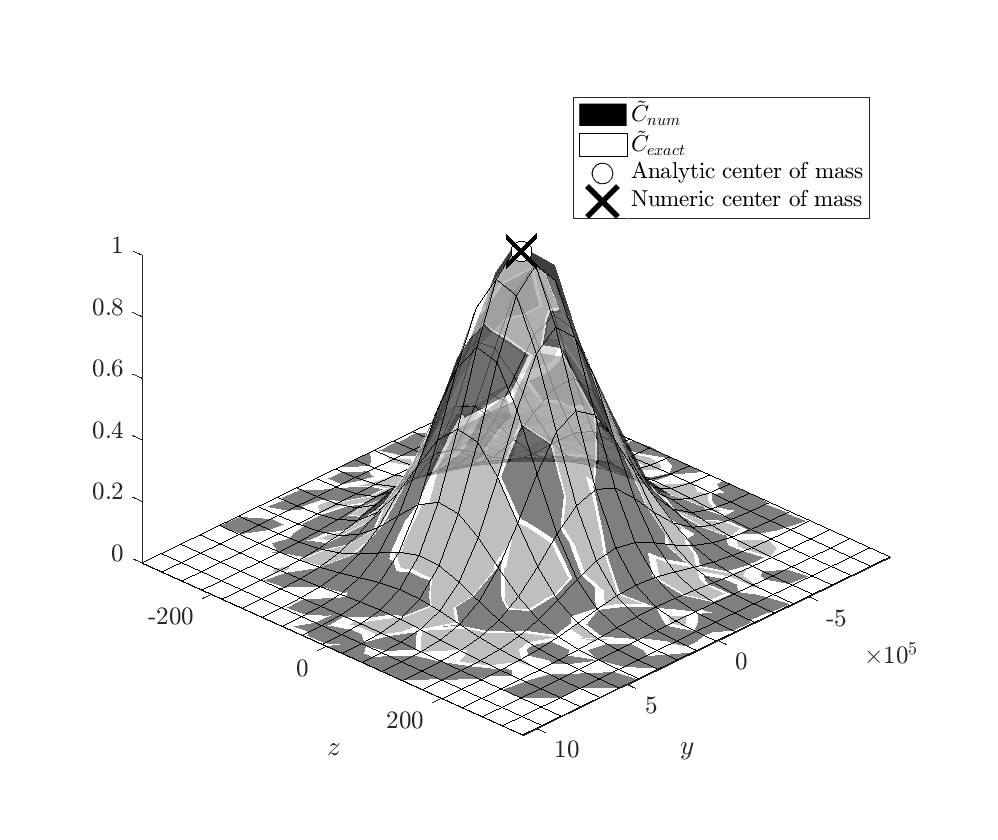
\includegraphics[width = \textwidth]{fig/testcase/testcase_surf.eps}
	\caption{Comparison of the concentrations obtained analytically and numerically. The "centers of mass" of the concentration obtained numerically (black cross) and numerically (white bullet) are also shown on the figure.}
	\label{fig:testcase_surf}
\end{figure}
\begin{figure}[H]
	\centering
	\begin{subfigure}[b]{0.49\textwidth}
		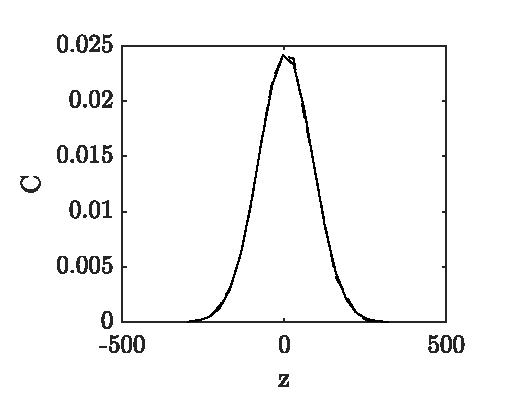
\includegraphics[width=\textwidth]{fig/testcase/testcase_fixedy.eps}
		\caption{$C_{num}(y_1+vT,z)$ and $C_{exact}(y_1+vT,z)$.}
		\label{fig:testcase_fixedy}
	\end{subfigure}
	\begin{subfigure}[b]{0.49\textwidth}
		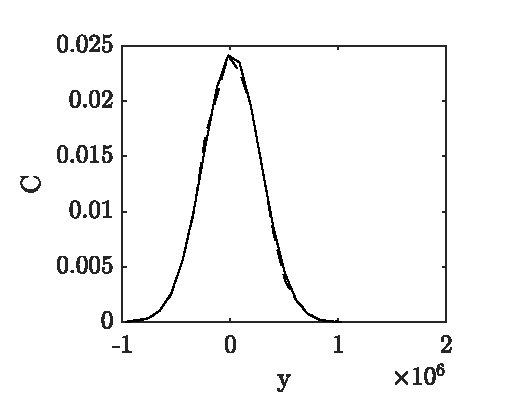
\includegraphics[width=\textwidth]{fig/testcase/testcase_fixedz.eps}
		\caption{$C_{num}(y,z_1+wT)$ and $C_{exact}(y,z_1+wT)$.}
		\label{fig:testcase_fixedz}
	\end{subfigure}
	\caption{Cut of the concentrations at fixed $y = r_{y,exact}$ and at fixed $z = r_{z,exact}$. The dashed line represent $C_{num}$ and the continuous line is for $C_{exact}$.}
\end{figure}

%-------------------------------------------RESULTS CASE 2-----------------------------------------------------------------------%
\subsection{Test case 2}
Figure \ref{fig:testcaseSI_surf} shows a comparison between the numerical result and the analytical solution for the (normalized) concentrations for test case 2. Since we do not have analytical expressions of the center of mass and of the variance for this test case, the "exact" values are approximated numerically thanks to the analytical expression of the concentration. Figures \ref{fig:testcaseSI_fixedy} and \ref{fig:testcaseSI_fixedz} represent respectively a cut of the concentrations at fixed $y = r_{y,exact}$ and along the boundary $z = 0$. The big picture about test case 2 is the presence of a boundary with no-through condition. A first verification is to check if all the particles are still in the domain, which is indeed the case. Although this might seem trivial here, it is sometimes a real challenge to ensure that no particle crosses the boundary, especially for geometrically complex domains. Besides, one can see on figure \ref{fig:testcaseSI_fixedz} that the concentration profile is well approximated along the boundary. Indeed, the maximal local error at the boundary is
\begin{equation}
	\|C_{exact}(y,0)-C_{num}(y,0)\|_{\infty} = 3.53\e{-4}, 
\end{equation}
The maximal local error on the whole domain is 
\begin{equation}
	\|C_{exact}-C_{num}\|_{\infty} = 1.097\e{-3}.
\end{equation}
The centers of mass are located at
\begin{equation}
	\b r_{exact} = (1.26\e{4},5.06\e{3}) \mbox{ [$m$],}\quad \b r_{num} = (1.10\e{4},5.05\e{3}) \mbox{ [$m$]}.
\end{equation}
The relative error is
\begin{equation}
	\b e_r = \left \lvert \frac{\b r_{exact}-\b r_{num}}{\b r_{exact}} \right \rvert =  \left(1.29\e{-1}, 1.825\e{-3}\right).
\end{equation}
The 2-norm of the relative error is
\begin{equation}
	\| \b e_r \|_2 = 1.29\e{-1}.
\end{equation}
This can be seen as a quantification of the error on advection. To quantify the error on diffusion, we compute the variance of the concentration :
\begin{equation}
	\sigma^2_{exact} = 6.39\e{10} \mbox{ [$m^2$],}\quad \sigma^2_{num} = 6.35\e{10} \mbox{ [$m^2$].}
\end{equation}
The relative error is
\begin{equation}
	e_{\sigma^2} = \left \lvert \frac{\sigma^2_{exact}-\sigma^2_{num}}{\sigma^2_{exact}}\right \rvert = 4.85\e{-3}.
\end{equation}
\begin{figure}[H]
	\centering
	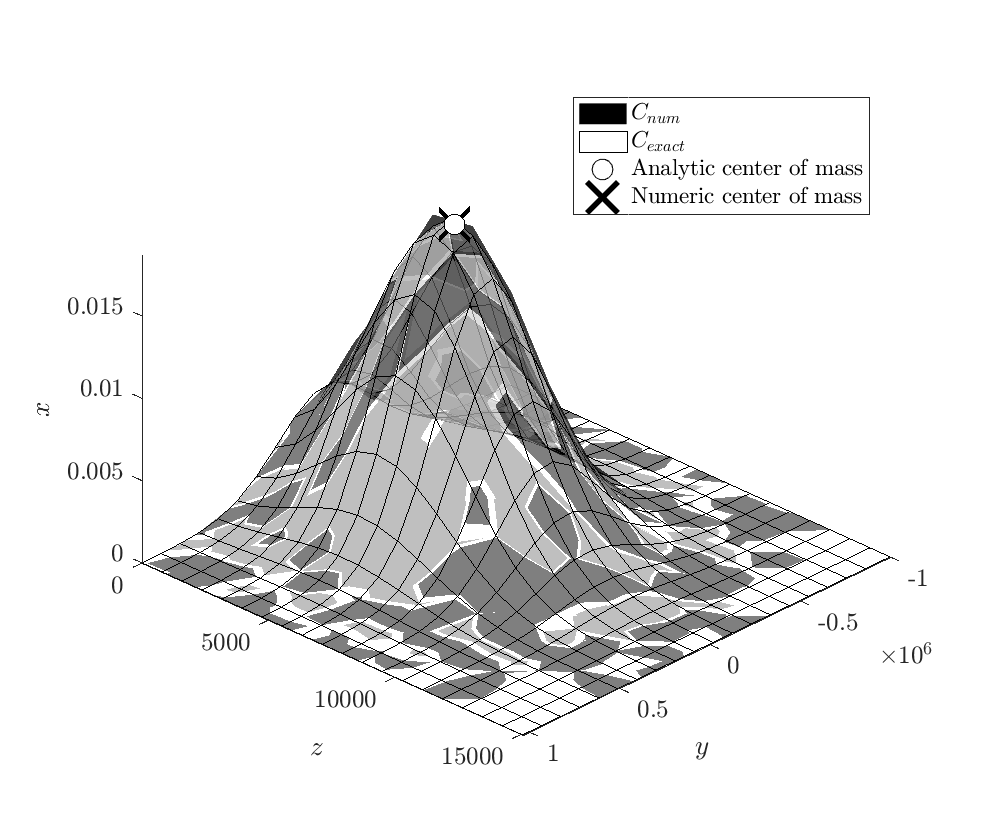
\includegraphics[width = \textwidth]{fig/testcase/testcaseSI_surf.eps}
	\caption{Comparison of the concentrations obtained analytically and numerically. The "centers of mass" of the concentration obtained numerically (black cross) and numerically (white bullet) are also shown on the figure.}
	\label{fig:testcaseSI_surf}
\end{figure}
\begin{figure}[H]
	\centering
	\begin{subfigure}[b]{0.49\textwidth}
		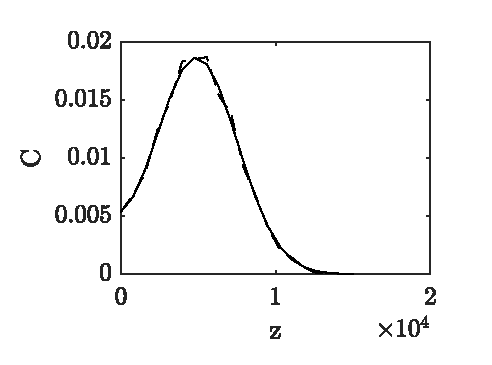
\includegraphics[width=\textwidth]{fig/testcase/testcaseSI_fixedy.eps}
		\caption{$C_{num}(y_1+vT,z)$ and $C_{exact}(y_1+vT,z)$.}
		\label{fig:testcaseSI_fixedy}
	\end{subfigure}
	\begin{subfigure}[b]{0.49\textwidth}
		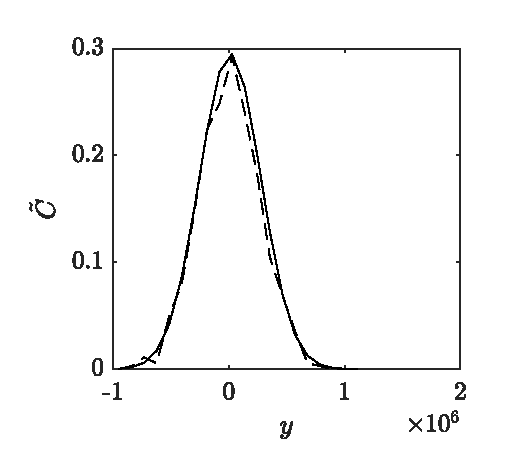
\includegraphics[width=\textwidth]{fig/testcase/testcaseSI_fixedz.eps}
		\caption{$C_{num}(y,z_1+wT)$ and $C_{exact}(y,z_1+wT)$.}
		\label{fig:testcaseSI_fixedz}
	\end{subfigure}
	\caption{Cut of the concentrations at fixed $y = r_{y,exact}$ and at fixed $z = r_{z,exact}$. The dashed line represent $C_{num}$ and the continuous line is for $C_{exact}$.}
\end{figure}